% TEMPLATE AUTHOR: https://bitbucket.org/m_by/fiit-stu-thesis-template-for-latex
% EDIT: Jozef Gáborík 


% SETTINGS - LATEX
% to change name, title, supervisor etc. go to preamble/preamble.tex
\newcommand{\myFontSize}[0] {12pt}
\newcommand{\mySpacing}[0] {1.5}
\newcommand{\myBibliography}[0] {bib/refs, appendices/refs1}
\documentclass[\myFontSize,a4paper,twoside,openright,english]{book}
\setlength{\headheight}{14.5pt}

\usepackage[utf8]{inputenc}
\usepackage[T1]{fontenc}
\usepackage[english]{babel}
\usepackage[a4paper]{geometry}
\usepackage[
    left = \glqq,% 
    right = \grqq,% 
    leftsub = \glq,% 
    rightsub = \grq%
]{dirtytalk}

% SETTINGS - NAMES
\newcommand{\myTitle}[0] {Simulator for instruction pipelining}
\newcommand{\myName}[0] {Bc. Martin Dinja}
\newcommand{\mySupervisor}[0] {Ing. Ján Hudec PhD.}
\newcommand{\myEvidenceNumber}[0] {FIIT-3028-52076}
\newcommand{\myDate}[0] {Máj 2025}
\newcommand{\myStudyProgram}[0] {Software Engineering}
\newcommand{\myDegreeCourse}[0] {9.2.5 Software Engineering}
\newcommand{\myInstitute}[0] {Institute of Informatics and Software Engineering, FIIT STU, Bratislava}

\usepackage[parfill]{parskip}
\usepackage{enumitem}

\usepackage{graphicx}
\usepackage{float}
\usepackage{longtable}
\usepackage{setspace}

% Spacing
\setstretch{\mySpacing}

\setcounter{secnumdepth}{3}
\setcounter{tocdepth}{3}

\usepackage{tabularx}
\newsavebox\mybox
\usepackage{fancyhdr}
\pagestyle{fancy}
\lhead{\nouppercase{\leftmark}}
\chead{}
\rhead{}
\lfoot{}
\cfoot{\thepage}
\rfoot{}


%style=iso-numeric
%style=authortitle-dw
\usepackage[backend=bibtex,defernums=true]{biblatex}
\defbibheading{references}[References]{ 
  \chapter*{#1}
  \markboth{#1}{#1}
}
\bibliography{\myBibliography}


% Listing as figure
%\usepackage{libs/minted}
%\usepackage[section]{minted}

\usepackage{listing}

% openright does not work :(
\let\tmp\oddsidemargin
\let\oddsidemargin\evensidemargin
\let\evensidemargin\tmp
\reversemarginpar

\usepackage{lscape}
\usepackage{afterpage}

\usepackage{lipsum}

\begin{document}
% Preamble

% Minted
% pygmentize -L styles
% \usemintedstyle{autumn}

% Title page

\begin{center}
\thispagestyle{empty}
{\Large Slovenská technická univerzita v Bratislave}
\par\end{center}{\Large \par}

\begin{center}
{\Large Fakulta informatiky a informačných technológií}
\par\end{center}{\Large \par}

\smallskip{}

\begin{center}
\myEvidenceNumber
\par\end{center}
\vfill{}

\begin{center}
\textbf{\Large \myName}
\par\end{center}{\Large \par}

\medskip{}


\begin{center}
\textbf{\LARGE \myTitle }
\par\end{center}{\huge \par}

\medskip{}


\begin{center}

{\Large Bakalárska práca}
\par\end{center}{\Large \par}

\vfill{}

Vedúci práce: \mySupervisor

\medskip{}
\myDate

\pagenumbering{roman}

\newpage
\thispagestyle{empty}
\mbox{}
\newpage



\begin{center}
\thispagestyle{empty}
{\Large Slovenská technická univerzita v Bratislave}
\par\end{center}{\Large \par}

\begin{center}
{\Large Fakulta informatiky a informačných technológií}
\par\end{center}{\Large \par}

\smallskip{}

\begin{center}
\myEvidenceNumber
\par\end{center}
\vfill{}

\begin{center}
\textbf{\Large \myName}
\par\end{center}{\Large \par}

\medskip{}


\begin{center}
\textbf{\LARGE \myTitle }
\par\end{center}{\huge \par}

\medskip{}


\begin{center}

{\Large Bakalárska práca}
\par\end{center}{\Large \par}

\vfill{}

Študijný program: \myStudyProgram

Študijný odbor: \myDegreeCourse

Miesto vypracovania: \myInstitute

Vedúci práce: \mySupervisor

\medskip{}

\myDate


\newpage
\thispagestyle{empty}
\mbox{}
\newpage



% Annotation
\thispagestyle{empty}

\section*{Annotation}

\begin{minipage}[t]{1\columnwidth}%
Slovak University of Technology Bratislava 

FACULTY OF INFORMATICS AND INFORMATION TECHNOLOGIES

Degree Course: \myStudyProgram
\newline

Author: \myName

Diploma Thesis: \myTitle

Supervisor: \mySupervisor

\myDate%
\end{minipage}

\bigskip{}

The aim of this thesis is to address the problem of outdated and difficult to use simulators for instruction pipelining, -mainly the archaic MIPSim used by the Principles of Computer Engineering course at FIIT STU- by introducing a new simulator. It is designed to be used by students and teachers to better understand the concept of instruction pipelining and its inner workings. This thesis analyzes the instruction pipelining concept, the existing simulators, their shortcomings, and proposes a new simulator that addresses those shortcomings, and describes its implementation. The new simulator is implemented using modern web technologies and is designed to be user friendly and easy to use. The simulator is evaluated by students and teachers to determine its usability and effectiveness in teaching and learning instruction pipelining.


\newpage{}\thispagestyle{empty}

\newpage
\thispagestyle{empty}
\mbox{}
\newpage

\thispagestyle{empty}
\section*{Anotácia}

\begin{minipage}[t]{1\columnwidth}%
Slovenská technická univerzita v Bratislave

FAKULTA INFORMATIKY A INFORMAČNÝCH TECHNOLÓGIÍ

Študijný program: Informatika
\newline

Autor: \myName

Bakalárska práca: Simulator na prúdove spracovanie inštrukcií

Vedúci bakalárskej práce: \mySupervisor

Máj 2025
\end{minipage}

\bigskip{}

Cieľom tejto práce je vyriešiť problém zastaraných a ťažko použiteľných simulátorov pre prúdove spracovanie inštrukcií -hlavne archaického MIPSimu používaného v predmete Základy počítačového inžinierstva na FIIT STU- zavedením nového simulátora. Je navrhnutý tak, aby ho mohli používať študenti a učitelia na lepšie pochopenie koncepcie prúdoveho spracovania inštrukcií a jeho vnútorného fungovania. Táto práca analyzuje koncept prúdoveho spracovania inštrukcií, existujúce simulátory a ich nedostatky. Navrhuje nový simulátor, ktorý tieto nedostatky rieši, a opisuje jeho implementáciu. Nový simulátor je implementovaný pomocou moderných webových technológií a je navrhnutý tak, aby bol užívateľsky prívetivý a ľahko použiteľný. Simulátor je hodnotený študentmi a učiteľmi s cieľom určiť jeho použiteľnosť a účinnosť pri výučbe a učení sa pipelingu inštrukcií.

\newpage{}\thispagestyle{empty}\medskip{}


\newpage{}


\thispagestyle{empty}
\mbox{}
\newpage



% Acknowledgements
\thispagestyle{empty}
\section*{Acknowledgment}

I would like to express my gratitude to my supervisor, \mySupervisor, for his guidance, support, and patience throughout the course of this thesis.

\newpage
\thispagestyle{empty}
\mbox{}
\newpage

% Table of contents
\tableofcontents{}

% List of listings
%\listoffigures\newpage{}
%\renewcommand\listoflistingscaption{List of Listings}
%\listoflistings\newpage{}

% References segment
\begin{refsegment}

% Introduction
\clearpage\null
\chapter{Introduction}
\pagenumbering{arabic}


Instruction pipelining is an intrestingly simple concept... But to truly understanding this idea of parallelism can be challenging. It feels like reading music without ever hearing a song. The flow, the stalls, the hazards—they were words without a melody. And many tools that try to help with visualizing these notes are outdated in today's day and age.
This thesis was born out of a desire to transform that silence into a beautiful symphony, crafting an instrument that would allow learners to not just see, but experience the song of instruction pipelining.

In contrast to how a non pipelined processor works, a pipelined processor executes multiple instructions simultaneously. One at each stage of the pipeline. This allows for a higher throughput of instructions, but also introduces a new set of challenges.

The problem is that there is no modern, user-friendly tool that allows for the visualization of instruction pipelining in a way that is easy to understand. Most tools are either outdated, or too complex to use, which makes it difficult for students to learn about this interesting topic.

To bridge the gap. This thesis aims to analyze existing solutions, identify their limitations, and propose a comprehensive solution in the form of a web-based instruction pipeline simulator
The paper is organized as follows: Chapter 2 provides an analysis of existing solutions, Chapter 3 presents the proposed solution, Chapter 4 describes the implementation of the solution, Chapter 5 discusses the verification of the solution, and Chapter 6 concludes the paper with a summary and future work.




% Analysis
\clearpage\null
\chapter{Analysis}

\section{Background}
\subsection{Historical Context}
Pipelining as a concept existed far before even the first definitive RISC processor was developed.
The machines like the IBM 7030(1959) and CDC 6600(1964) we're the first general-purpose pipelined machines. After that pipelining was constantly improving and by the 1980s most of the terminology and concepts we use today were already established\cite{pantazi2013history}. In the 1970s and 1980s in response to the increasing complexity of CISC(Complex Instruction Set Computer) processors researchers realized that simplifying the instruction set could lead to better performance. That is because in CISC \enquote{25\% of the instructions in the instructions' set make up 95\% of the execution time. This means that about 75\% of the hardware-sup-ported instructions often are not used at all}\cite{jamil1995risc}. This insight is how the first RISC(Reduced Instruction Set Computer) projects were developed\cite{aletan1992overview} and they were originally designed to have pipelining in mind\cite{pantazi2013history}. The first RISC system - as considered by Michael J. Flynn - was the IBM 801\cite{flynn1995computer}, which was developed in the early 1980s in an effort to make a digital telephone switch able to handle 300 phone calls per second\cite{cocke1990evolution}. The most notable mention especially  in the context of this thesis would be the Stanford MIPS architecture developed by John L. Hennessy and David A. Patterson in the 1980s. Its main goal was to attain high performance in the execution of compiled code by closely relating the instruction to the microcode instructions\cite{hennessy1982mips}. MIPS is still used today in embedded systems, networking, and educational settings. For a more detailed overview of the history of pipelining and RISC, see "The history and use of pipelining computer architecture" by Pantazi et al.\cite{pantazi2013history} and "The evolution of RISC technology at IBM" by Cocke and Markstein et al.\cite{cocke1990evolution}.

\subsection{RISC vs CISC}
The main difference between RISC and CISC is the complexity of the instruction set. CISC processors have complex instructions requiring multiple clock cycles and the use of microcode to execute, while RISC processors have simple instructions that can be executed in a single clock cycle\cite{jamil1995risc}. This makes RISC processors easier to implement and optimize, as well as more efficient in terms of power consumption and performance. And since the simple instructions can be executed in a single clock cycle, this makes RISC processors more suitable for pipelining. CISC processors, on the other hand, are more difficult to pipeline due to the complexity of the instructions. However, when it comes to program size, Compiled CISC programs are generally smaller than compiled RISC programs, because CISC instructions are more powerful and can perform more operations in a single instruction\cite{jamil1995risc}. This is why CISC processors are still used in many applications, such as desktop computers and servers, because of the backwards compatibility with older software and the ability to perform complex operations in a single instruction. RISC processors, on the other hand, are more commonly used in embedded systems, mobile devices, and other applications where power consumption and performance are critical\cite{ryzhyk2006arm}.

\section {Instruction Pipelining}\label{sec:pipelining}

\subsection {Introduction}\label{sec:pipelining_intro}
Pipelining is a method used to enhance a processor's throughput by overlapping the execution phases of multiple instructions. By dividing the execution of an instruction into several stages and executing multiple instructions concurrently, the processor can handle several instructions simultaneously, thereby increasing its throughput\cite{olanrewaju2017design}. Figure \ref{fig:pipeline} illustrates the concept of pipelining.

\begin{figure}[H]
    \centering
    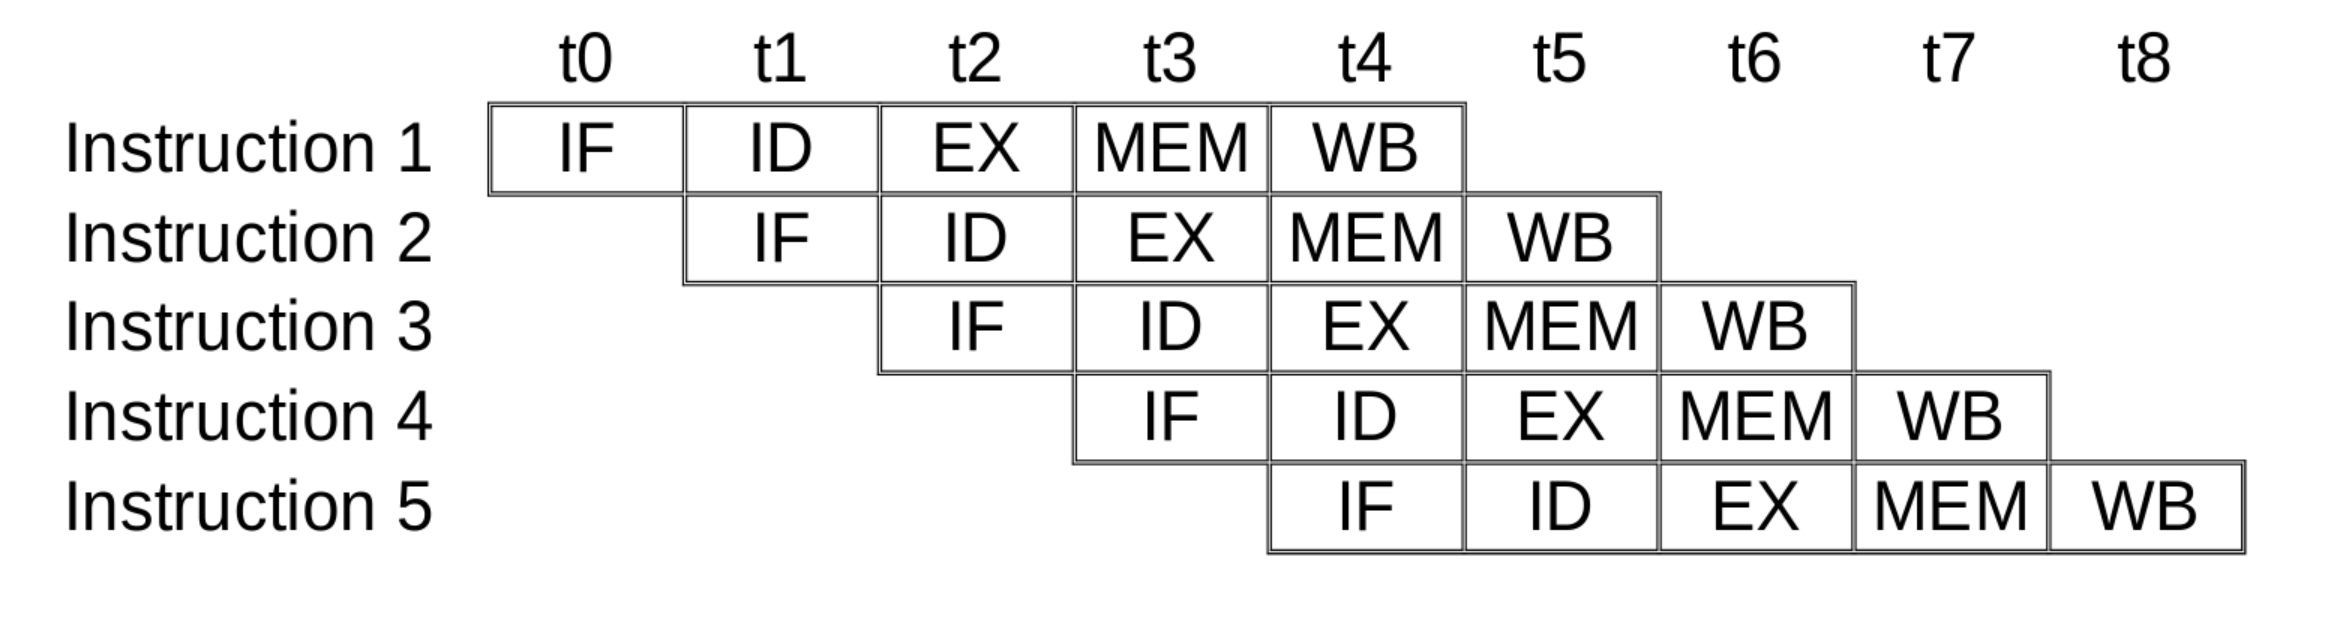
\includegraphics[width=0.8\textwidth]{assets/images/pipeline.png}
    \caption{Pipelining} 
    \label{fig:pipeline} 
\end{figure}

As seen in Figure \ref{fig:pipeline}, this example pipeline is divided into five stages, and looking at any column we can see what instruction would be in what stage at the given time. For example, at time $t_3$, instruction 1 is in the MEM stage, instruction 2 is in the EX stage, instruction 3 is in the ID stage and instruction 4 is in the IF stage. This is how pipelining works and what is meant by overlapping the execution phases of multiple instructions. The stages of the pipeline are described in the next section \ref{sec:pipeline_stages}.


\subsection {Instruction Pipeline Stages}\label{sec:pipeline_stages}
The classical RISC pipeline consists of five stages: instruction fetch, instruction decode, execute, memory access, and write-back \cite{enwiki:1255528196}\cite{he2023survey}. 

\begin{itemize}
     \item \textbf{Instruction Fetch (IF)}: Fetches the instruction from memory using the program counter, which is then incremented.
     \item \textbf{Instruction Decode (ID)}: Decodes the instruction to determine the operation and fetches operands from the register file.
     \item \textbf{Execute (EX)}: Performs the operation on the fetched operands.
     \item \textbf{Memory Access (MEM)}: Accesses memory for load/store instructions; otherwise, bypassed.
     \item \textbf{Write-back (WB)}: Writes the result back to the destination register.
\end{itemize}


\subsection {Pipeline Stalls}\label{sec:pipeline_stalls}
Pipeline stalls, also known as pipeline bubbles, are empty stages that occur when an instruction cannot move on to the next stage due to a hazard or dependency. Stalls decrease the efficiency of the pipeline and result in wasted clock cycles. \cite{patterson1994computer}.

\subsection {Pipeline Hazards}\label{sec:pipeline_hazards}
A hazard is a condition that occurs when the pipeline cannot execute the next instruction in the cycle, or its execution will lead to unintended behavior. There are three types of hazards: structural, data, and control hazards\cite{olanrewaju2017design}.

\subsubsection {Structural Hazards}\label{sec:structural_hazards}
Structural hazards occur when the hardware cannot support the combination of instructions in the pipeline. For example, if two instructions require the same hardware resource, such as the register control unit.
This stalls the pipeline or corrupts a result.
There are multitude of ways to avoid them, such as scheduling instructions to avoid conflicts, or adding extra hardware to support multiple instructions at once\cite{proebsting1994detecting}.
\subsubsection {Data Hazards}\label{sec:data_hazards}
Data hazards occur when an instruction depends on a previous instruction. There are four main types of data hazards: read-after-write (RAW), write-after-read (WAR), write-after-write (WAW), and read-after-read (RAR).

\textbf{Read-After-Write (RAW)}: Also known as a true dependency it occurs when an instruction reads a register before a previous instruction writes to it.\newline
\textbf{Example}: Consider the following instructions:
\begin{verbatim}
add $t0, $t1, $t2
sub $t3, $t0, $t4   
\end{verbatim}
`add` writes to register \$t0, and `sub` reads from it, so the `sub` instruction cannot be executed until the `add` instruction has completed.\newline
\textbf{Solution}: Use techniques such as forwarding (or bypassing), where we add extra paths to the pipeline to allow the result of an instruction to be forwarded to the next instruction that needs it.

\textbf{Write-After-Read (WAR)}: Also known as an anti dependency it occurs when an instruction writes to a register after a previous instruction reads from it.\newline
\textbf{Example}: Consider the following instructions:
\begin{verbatim}
add $t1, $t0, $t2
sub $t0, $t3, $t4
\end{verbatim}
`sub` tries to write to register \$t0 after `add` has read from it.
\textbf{Solution}: This hazard is rare in RISC architectures and nonexistent in the classical RISC pipeline since reads are done in the ID stage and writes in the WB stage. Otherwise, it can be avoided due to the use of register renaming, which ensures that each instruction has a unique destination register. 

\textbf{Write-After-Write (WAW)}: Also know as an output dependency it occurs when two instructions write to the same register.\newline
\textbf{Example}: Consider the following instructions:
\begin{verbatim}
add $t0, $t1, $t2
sub $t0, $t3, $t4
\end{verbatim}
`sub` tries to write to register \$t0 before `add` has completed writing to it.\newline
\textbf{Solution}: Similar to WAR hazards, nonexistent in the classical RISC pipeline since register writes are in order. Otherwise, register renaming can be used to avoid WAW hazards by ensuring that each write operation targets a unique register.

\textbf{Read-After-Read (RAR)}: Occurs when read operations are performed sequentially.\newline
Further detail is unnecessary because it is immediately obvious that this hazard is not possible in classical RISC pipelines, as reads do not change the state of the registers.



\subsubsection {Control Hazards}\label{sec:control_hazards}
Control hazards occur when the processor cannot determine the instruction to fetch next due to a branch instruction changing the program counter. This can lead to incorrect execution of instructions and wasted clock cycles. There are several techniques to mitigate control hazards, such as branch prediction, delayed branching and branch target buffers.\cite{pandey2016study}


\section {MIPS}\label{sec:mips}
\subsection{Overview}
MIPS, which stands for Microprocessor without Interlocked Pipeline Stages, is a RISC architecture that has made a significant impact in the world of computing. Developed by MIPS Tech LLC\cite{mipscompany}, a company founded in 1984 by Stanford University researchers including John L. Hennessy and David A. Patterson, MIPS has become a cornerstone in embedded systems, networking, and education. Its load/store architecture and 5-stage pipeline, detailed in section \ref{sec:mips_pipeline}, make it a model of simplicity and efficiency. This straightforward design is why MIPS is an excellent choice for teaching computer architecture. Especially because "Computer Organization and Design" by Patterson and Hennessy\cite{patterson1994computer}, which can be considered the bible of computer architecture, uses MIPS as the primary example throughout the book. Over the years, MIPS has evolved through several versions, including MIPS I, II, III, IV, V, MIPS32, and MIPS64, each adding new features and capabilities. In this section, we'll focus on the MIPS I architecture to grasp the fundamental concepts of the MIPS architecture and the inner workings of the MIPS pipeline.

\subsection{Registers}
The MIPS architecture has 32 32-bit general-purpose registers and 32 floating point registers, numbered from \$0 to \$31 and \$f0 to \$f31 respectivly. For integer multiplication and division, there are two special registers, HI and LO, which store the high and low 32 bits of the result. And of course the program counter, which is used to store the address of the next instruction to be executed. The MIPS registers are used to store data, addresses, and control information, and are accessed using load and store instructions. The registers are divided into several categories, each with a specific purpose.
\subsubsection{General-Purpose Registers}
General purpose registers are used to store data and perform arithmetic and logical operations, pass arguments to functions, store return values, and hold temporary values.
Even though these registers could be used for any purpose, there are conventions on how they should be used:
\begin{table}[h]
    \centering
        \begin{tabular}{|c|c|l|}
        \hline
        \textbf{Register Number} & \textbf{Name} & \textbf{Description} \\ \hline
        \$0 & \$zero & Constant value 0 \\ \hline
        \$1 & \$at & Assembler temporary \\ \hline
        \$2-\$3 & \$v0-\$v1 & Function return values \\ \hline
        \$4-\$7 & \$a0-\$a3 & Function arguments \\ \hline
        \$8-\$15 & \$t0-\$t7 & Temporary registers \\ \hline
        \$16-\$23 & \$s0-\$s7 & Saved registers \\ \hline
        \$24-\$25 & \$t8-\$t9 & More temporary registers \\ \hline
        \$26-\$27 & \$k0-\$k1 & Reserved for OS kernel \\ \hline
        \$28 & \$gp & Global pointer \\ \hline
        \$29 & \$sp & Stack pointer \\ \hline
        \$30 & \$fp & Frame pointer \\ \hline
        \$31 & \$ra & Return address \\ \hline
        \end{tabular}
    \caption{MIPS Registers and Their Names}
    \label{tab:mips_registers}
\end{table}
\subsubsection{\$at Register}
The \$at register is reserved for the assembler to store temporary values during translation of high-level code to machine code. It is not preserved across function calls.

\textbf{\$v0-\$v1 Registers}\newline
These registers store function return values.

\textbf{\$a0-\$a3 Registers}\newline
These registers pass arguments to functions. 

\textbf{\$t0-\$t9 Registers}\newline
Temporary registers for storing values that do not need to be preserved across function calls.

\textbf{\$s0-\$s7 Registers}\newline
Saved registers that preserve values across function calls.

\textbf{\$k0-\$k1 Registers}\newline
Reserved for the operating system kernel.

\textbf{\$gp Register}\newline
The global pointer register, used to store the base address of the global data segment. It is preserved across function calls.

\textbf{\$sp Register}\newline
The stack pointer register, which tracks the top of the stack. It is preserved across function calls.

\textbf{\$fp Register}\newline
The frame pointer register, used to access the current stack frame, local variables, and function arguments. It is preserved across function calls.

\textbf{\$ra Register}\newline
The return address register, which stores the address to return to after a function call. It is preserved across function calls.

\subsubsection{Floating Point Registers}\label{sec:floating_point_registers}
MIPS supports the IEEE 754 single precision and double precision formats\cite{patterson1994computer} where the single precision format is 32 bits long and the double precision format is 64 bits long. A double precision floating point register is really an even-odd pair of single precision registers\cite{patterson1994computer}. For example \$f2 and \$f3 together form a double precision register referred to as \$f2, and same for all the other even-odd pairs. The floating point registers are used for floating point operations and are not preserved across function calls. They are numbered from \$f0 to \$f31 and don't have a definitive name and usage conventions. MIPS does not directly support floating point arithmetic\cite{hennessy1982mips}, instead, these operations are implemented with integer operations or by using a coprocessor.

\subsubsection{HI and LO Registers}
The HI and LO registers are used to store the high and low 32 bits of the result of a multiplication or division operation. The HI register stores the high 32 bits, and the LO register stores the low 32 bits. These registers are not preserved across function calls.

\subsection{Instruction Formats}
The MIPS instruction set consists of three instruction formats: R-type, I-type, and J-type. Each format is used for different types of instructions, such as arithmetic, logical, and control instructions. The R-type format is used for arithmetic and logical instructions, the I-type format is used for immediate instructions, and the J-type format is used for jump instructions. The machine format of each instruction is 32 bit.


\subsubsection{R-type Format}
The R-type format is used for arithmetic and logical instructions that operate on registers. It takes 3 arguments: the destination register(rd), the source register(rs), and the second source register(rt). Example:
\begin{verbatim}
    add rd, rs, rt
\end{verbatim}

The machine format of the instruction is as follows:
\begin{table}[H]
    \centering
    \begin{tabular}{|c|c|c|c|c|c|}
    \hline
    \textbf{opcode} & \textbf{rs} & \textbf{rt} & \textbf{rd} & \textbf{shamt} & \textbf{funct} \\ \hline
    6 bits         & 5 bits     & 5 bits     & 5 bits     & 5 bits        & 6 bits        \\ \hline
    \end{tabular}
    \caption{R-type Format}
    \label{tab:r_type_format}
\end{table}
\begin{itemize}
    \item \textbf{opcode}: The operation code.
    \item \textbf{rs}: The source register.
    \item \textbf{rt}: The second source register.
    \item \textbf{rd}: The destination register.
    \item \textbf{shamt}: The shift amount.
    \item \textbf{funct}: The function code.
\end{itemize}
The interesting thing in the R-type format is that the opcode is always 0, and the funct field is used to determine the operation to be performed. And shamt is used in shift instructions such as sll, srl, sra.

\subsubsection{I-type Format}
The I-type format is used for immediate instructions that operate on registers and immediate values. It has 3 arguments: the source register(rs), the destination register(rd), and the immediate value. Example:
\begin{verbatim}
    addi rd, rs, imm
\end{verbatim}

The machine format of the instruction is as follows:
\begin{table}[H]
    \centering
    \begin{tabular}{|c|c|c|c|}
    \hline
    \textbf{opcode} & \textbf{rs} & \textbf{rt} & \textbf{imm} \\ \hline
    6 bits         & 5 bits     & 5 bits     & 16 bits     \\ \hline
    \end{tabular}
    \caption{I-type Format}
    \label{tab:i_type_format}
\end{table}

\begin{itemize}
    \item \textbf{opcode}: The operation code.
    \item \textbf{rs}: The source register.
    \item \textbf{rt}: The destination register.
    \item \textbf{imm}: The immediate value.
\end{itemize}
Other than just performing arithmetic operations, the I-type format is also used for load and store instructions, and branch instructions. \newline
Examples:
\begin{verbatim}
    lw rt, imm(rs) # Load word
    sw rt, imm(rs) # Store word
    beq rs, rt, imm # Branch if equal
\end{verbatim}
The load and store instructions are the only instructions that have a different assembly syntax then the rest of the instructions.

\subsubsection{J-type Format}
The J-type format is used for jump instructions. It has only one argument: the jump address. Example:
\begin{verbatim}
    j addr
\end{verbatim}

The machine format of the instruction is as follows:
\begin{table}[H]
    \centering
    \begin{tabular}{|c|c|}
    \hline
    \textbf{opcode} & \textbf{addr} \\ \hline
    6 bits         & 26 bits      \\ \hline
    \end{tabular}
    \caption{J-type Format}
    \label{tab:j_type_format}
\end{table}

\begin{itemize}
    \item \textbf{opcode}: The operation code corresponding to the jump instruction.
    \item \textbf{addr}: The pseudo-direct address of the jump target. The 32-bit address is formed by shifting the 26 bit address left by 2 bits and concatenating the 4 most significant bits of the program counter.
\end{itemize}
The J-type format is used for jump and jump-and-link instructions. The jump-and-link instruction stores the return address in register \$ra before jumping to the target address.

\subsection{Assembly Language}
The conventional general notation for MIPS assembly language is as follows:
\begin{verbatim}
    label: instruction arg1, arg2, arg3
\end{verbatim}
The label is optional and is used to mark a specific location in the program. The instruction is the operation to be performed, and the arguments are the operands of the instruction. The arguments can be registers, immediate values, or memory addresses depending on the instruction. The arguments are separated by commas, and the instruction is followed by a newline character. The assembly language is case-insensitive, and whitespace is used to separate tokens. Comments can be added using the `\#` character, and the assembler ignores everything after it. The only exception to this rigid structure is the load and store instructions, which have a different syntax. Example: 
\begin{verbatim}
    lw rt, imm(rs)
    sw rt, imm(rs)
\end{verbatim}
The load instruction loads a word from memory at the address rs+imm and stores it in register rt. The store instruction stores the word in register rt to memory at the address rs+imm.

Of course an assembly language can be designed in any way, but this is the most common way MIPS assembly is written.

Instructions can be categorized into six groups: arithmetic, logical, comparison, data transfer, conditional branch, and unconditional jump. 

The arithmetic, logical and comparison instructions operate on registers and immediate values, while the data transfer instructions load and store data from memory. The conditional branch instructions change the program counter based on a condition, and the unconditional jump instructions jump to a specific address. Table \ref{tab:mips_instructions} shows examples of instructions from each group.
% Instructions table
\begin{table}[H]
    \centering
    \resizebox{\textwidth}{!}{
    \begin{tabular}{|c|c|c|}
    \hline
    \textbf{Group} & \textbf{Example Instruction} & \textbf{Description} \\ \hline
    Arithmetic & add rd, rs, rt & Add rs and rt and store the result in rd \\ \hline
    Logical & and rd, rs, rt & Bitwise AND of rs and rt and store the result in rd \\ \hline
    Comparison & slt rd, rs, rt & Set rd to 1 if rs < rt, 0 otherwise \\ \hline
    Data Transfer & lw rt, imm(rs) & Load word from memory at address rs+imm and store in rt \\ \hline
    Conditional Branch & beq rs, rt, label & Branch to label if rs and rt are equal \\ \hline
    Unconditional Jump & j addr & Jump to address addr \\ \hline
    \end{tabular}}
    \caption{Example MIPS Assembly Instructions for Each Group}
    \label{tab:mips_instructions}
\end{table}

There also exist exception handling instructions that are used to handle exceptions and interrupts. However, these are not used in the context of this thesis.

\subsection{MIPS Pipeline}\label{sec:mips_pipeline}
The MIPS pipeline consists of five stages: instruction fetch(IF), instruction decode(ID), execute(EX), memory access(MEM), and write-back(WB). Each stage is responsible for a specific part of the instruction execution process allowing it to overlap the execution of multiple instructions to improve performance and throughput. Here each stage will be described in detail according to the design shown in Figure \ref{fig:mips_pipeline}, which is the same design described in Patterson and Hennessy's "Computer Organization and Design" book\cite{patterson1994computer}.

\begin{figure}[H]
    \centering
    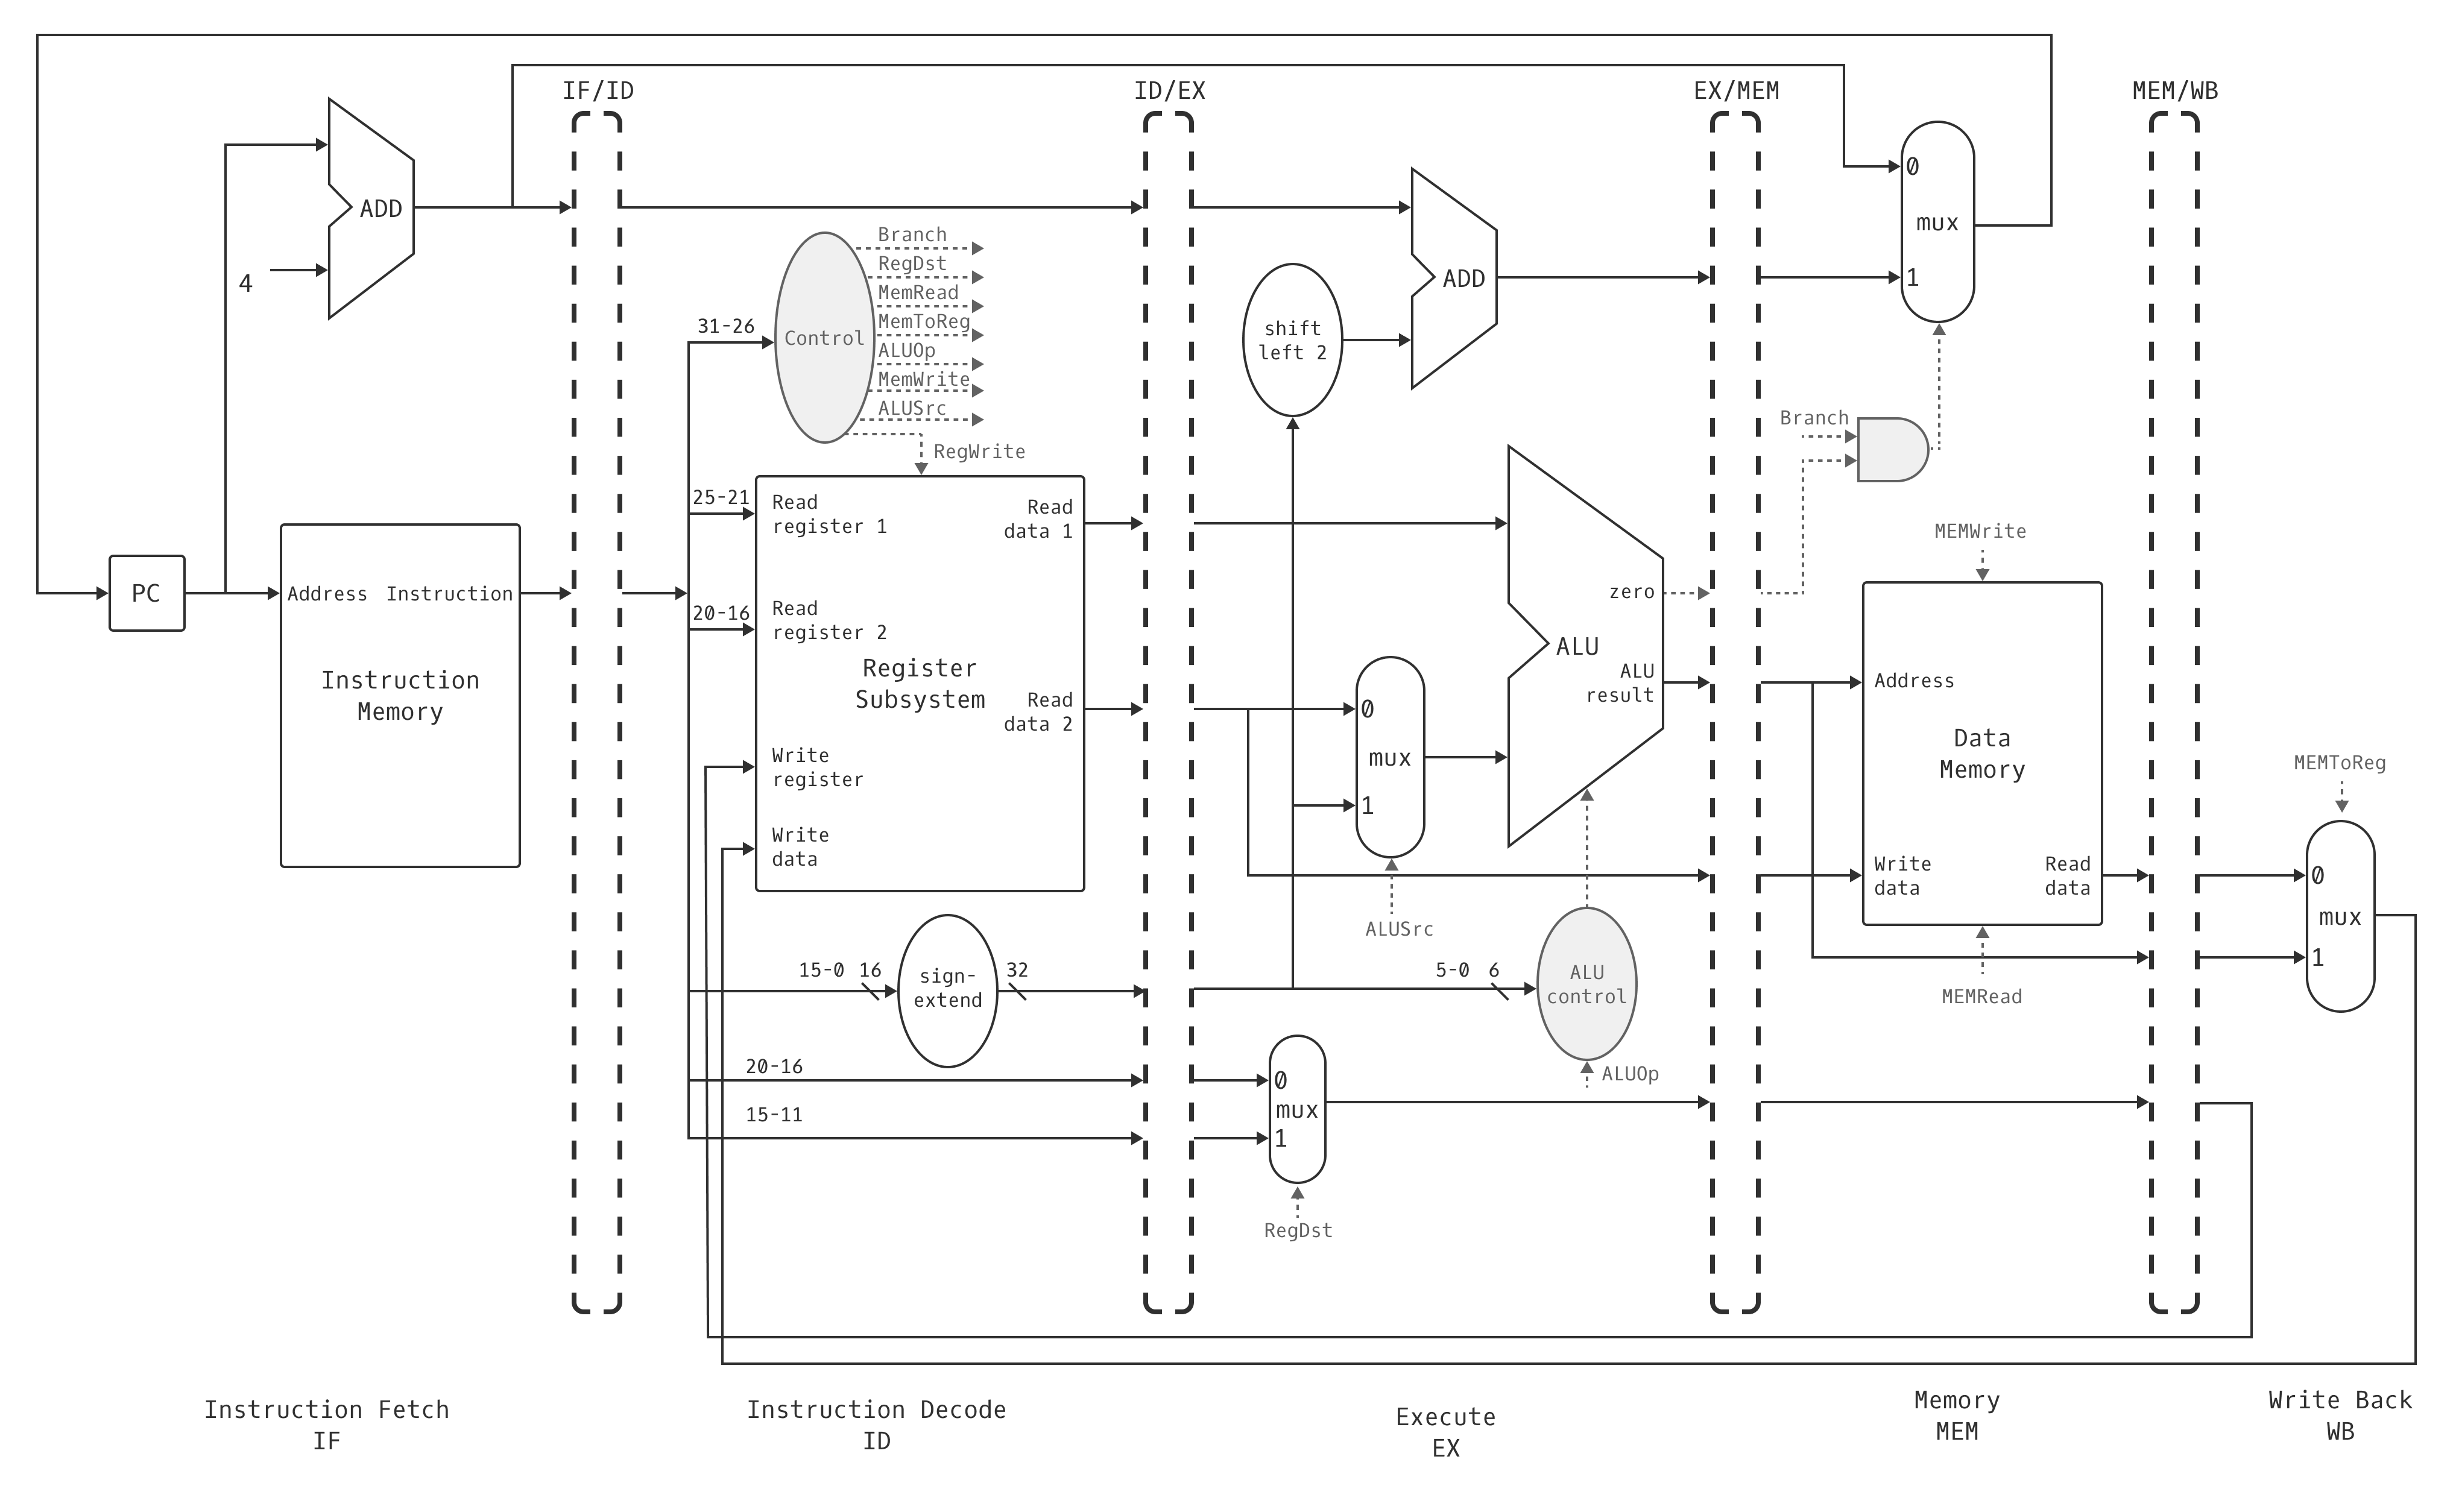
\includegraphics[width=1\textwidth]{assets/images/mips_pipeline.png}
    \caption{High-Level MIPS Pipeline Diagram with Control Unit}
    \label{fig:mips_pipeline}
\end{figure}

Figure \ref{fig:mips_pipeline} shows a high-level diagram of the MIPS pipeline with a control unit. It can get even more complex with the addition of forwarding and hazard detection units. But this current state is sufficient for the explanation of the pipeline stages.

Note: This design doesn't feature support for any J-type instructions and many other more complicated instructions for simplicity’s sake, and since they are not necessary to make a turning complete processor. Also, note that the J-type could be simulated by using an I-type branch instructions whose condition is a tautology. For example, $beq \$zero, \$zero, label$ would be equivalent to a jump instruction. MIPSIM is based on a design that handles jump instructions in such a way. But adding support for real unconditional jump instructions is not that difficult and will be covered in section \ref{sec:jump_capabilities}.



\subsubsection{Explanation of General Symbols}
Before diving into the details of each pipeline stage, it is important to understand the general symbols used in the pipeline diagram.

\textbf{Multiplexers (MUX):} The rounded rectangles represent multiplexers, which select one of the input signals based on a control signal. In the diagram there are only 2-to-1 multiplexers which only require one bit of control signal to select between two inputs. But in more complex designs, there could be 3 or 4-to-1 multiplexers which would require more bits of control signal.

\textbf{PC:} The small square box with PC written in it represents the program counter register, which stores the address of the next instruction to be fetched. 

\textbf{Stage Register}: The vertical dashed rectangles represent the stage registers. There are 4 of them, one for each transition between stages. A stage register stores the necessary values passed on from the previous stage to the next. It acts as a buffer between stages, allowing them to operate independently.

\textbf{Buses:} The lines connecting everything together, both dashed and solid, are buses, which carry data and control signals between components. A bus that carries data is a data bus, and a bus that carries control signals is a control bus.

\textbf{Control Signals:} The control signals are dashed lighter lines originating from the Control unit. They are generated by the control unit and determine which operations to perform at each stage. Which input should a multiplexer select, which operation should the ALU perform, etc.

\subsubsection{Instruction Fetch (IF) Stage}
The IF stage is responsible for fetching the instruction from memory using the program counter(PC), which is incremented by 4 after each fetch to point to the next instruction. After the instruction has been fetched from memory, it is saved to the IF/ID stage register to be passed to the next stage. 

\subsubsection{Instruction Decode (ID) Stage}
The ID stage is responsible for generating the control signals for the pipeline and decoding the instruction to determine the operation to be performed. 

The control unit receives the operation code of the instruction and generates the necessary control signals for the pipeline. The control signals are then passed to other stages through the stage registers and get used to control the multiplexers and other components in the pipeline. Note that the $RegWrite$ signal is not immediately 'applied' in the ID Stage; instead, it is carried all the way to the write-back stage, where it is then applied to the register subsystem. Since this diagram is a high-level diagram, this nuance is not shown to avoid making the diagram more cluttered, inconsistent, and harder to read.

The Register Subsystem is responsible for reading the registers $rs$ and $rt$ from the register file and passing the values to the EX stage. The register file is read using the $rs$ and $rt$ fields of the instruction, and the 32-bit values are passed to the EX stage through the ID/EX stage register.

The 16-bit immediate value is sign-extended to 32 bits and passed to the EX stage, as well as instruction bits from 20-16 and 15-11 which are used to detriment the write register used in the WB stage. This is because the I and R type instructions have their destination register at different positions in the instruction, so depending on the instruction type, the correct bits representing the destination register are passed to the WB stage.

\subsubsection{Execute (EX) Stage}
The EX stage is responsible for performing the operation on the operands received from the ID stage, calculating the branch address for branch instructions and determining the write register. 

The ALU performs the operation based on the ALUOp control signal, which makes its way to the ALU control unit. In this simplified design this signal has two bits which is all we need to be able to specify which operation to carry out to satisfy load/store instructions, branch instructions, or R-type arithmetic instructions.
\begin{table}[H]
    \centering
    \begin{tabular}{|c|c|c|}
    \hline
    \textbf{Instruction} &  \textbf{ALUOp} & \textbf{Function} \\ \hline
    Load/Store         & 00             & add  \\ \hline
    Branch            & 01             & subtract \\ \hline
    R-Type         & 10             & dependent on funct field \\ \hline
    \end{tabular}
    \caption{ALUOp Control Signal Values}
    \label{tab:aluop_values}
\end{table}

In more complex designs, the ALUOp signal would have more bits to allow for or, xor, and, etc. operations. This signal gets passed to the ALU control unit which generates the ALU control signal.

The ALU receives the two operands from the ID stage and performs the operation based on the ALU control signal. The ALU control also receives the $funct$ field or the lower 6 bits of the instruction, which is used to determine the operation to be performed by the ALU if the instruction is an R-type instruction. The result of the operation is then passed to the MEM stage through the EX/MEM stage register.

Branch address calculation is done by shifting the immediate value left by 2 bits and adding it to PC+4. The result is then passed to the MEM stage through the EX/MEM stage register.

And lastly, the write register is determined by the $RegDst$ control signal, which is passed to the MEM stage through the EX/MEM stage register.


\subsubsection{Memory Access (MEM) Stage}
The MEM stage is responsible for accessing memory for load and store instructions, and branching to the target address for branch instructions.

For load instructions, the data is read from memory at the address calculated in the EX stage and passed to the WB stage through the MEM/WB stage register. And for store instructions, the data is written to memory at the address calculated in the EX stage. The $MEMWrite$ and $MEMRead$ control signals determine whether to write or read from memory. If both are set to 0, the Data Memory unit is unused.

For branch instructions we have an AND gate that checks if the ALU Zero control signal is set to 1, and if it is, that means the condition that was evaluated in the EX stage is true. Based on that and the branch control signal, the multiplexer is sets either the branch address calculated in the EX stage or the PC+4 value as the new PC value.

\subsubsection{Write-Back (WB) Stage}
The WB stage is responsible for writing the result of the operation to the destination register. Using the $MEMToReg$ control signal, the multiplexer selects if the load data from the MEM stage or the ALU result from the EX stage should be written to the register file. The register file is then written to if the $RegWrite$ control signal is set to 1.

\subsection{Pipeline Hazards}
From the described pipeline stages, it would be immediately noticeable to someone somewhat versed in computer architecture that this pipeline design is very simple and doesn't handle any kind of hazards. The first issue that would arise is the structural hazard that could occur when reading and writing to the register file, since we have two stages that use the register subsystem at the same time. The second issue would be data hazards, especially read-after-write hazards, since the pipeline doesn't have any kind of forwarding or bypassing unit. And the third issue would be control hazards, since the pipeline doesn't have any kind of branch prediction or branch target buffer, and also since there is no flushing feature that would eliminate unwanted instructions that entered the pipeline before a branch instruction had the chance to update the PC. These are all issues that need to be addressed in a more complex pipeline design and far outpace the scope of this section. For a more detailed understanding of hazards and the design of pipelines that handle them, refer to "The Processor" chapter in "Computer Organization and Design" by Patterson and Hennessy\cite{patterson1994computer}.

However, it is still interesting to understand how these hazards would theoretically be handled in this pipeline design.

For structural hazards, the simplest solution is to perform write operations at the beginning of a clock cycle and read operations at the end of it. More technically, this means writing at the rising edge of the clock and reading at the falling edge.

For data hazards, one solution would beto stall the pipeline until the data is ready, which is slow, or a better solution would be adding a forwarding unit that would allow the result of an instruction to be forwarded to the next instruction that needs it. One case where forwarding cannot save the day is when an instruction tries to read a register following a load instruction that writes the same register\cite{patterson1994computer}. In that case in addition to a forwarding unit, a load-use hazard detection unit that would stall the pipeline until the load instruction has completed would be necessary.

For control hazards, solutions include stalling the pipeline or introducing a flushing mechanism to clear stage registers holding instructions that should not be executed. To improve the performance of determining when to flush, a branch prediction unit can be added. This unit predicts the outcome of branch instructions and decides whether to flush based on the prediction\cite{patterson1994computer}.

\subsection{Floating Point Operations}
It may have been noticed that floating point operations have not been discussed until now. This is because the MIPS architecture does not directly support floating point arithmetic, as mentioned in section \ref{sec:floating_point_registers}. Instead, floating point operations are typically handled by a coprocessor, such as the MIPS Floating Point Unit (FPU)\cite{mirapuri1992mips}.

The FPU is a specialized unit designed to handle floating point operations, communicating with the main processor through a coprocessor interface. It comes equipped with its own set of registers, control signals, and instructions tailored for floating point arithmetic\cite{patterson1994computer}. The MIPS architecture provides specific instructions for loading and storing floating point values, performing arithmetic operations, and converting between integer and floating point formats.

Typically, the FPU is either implemented as a separate chip or integrated into the main processor as a coprocessor. The main reason to have it on a separate chip is because of the lack of transistors in the 1980's. But since the early 1990s, microprocessors
have integrated floating point (and just about everything else) on chip\cite{patterson1994computer}.
\subsection{Expanding the design with more jump capabilities}\label{sec:jump_capabilities}
As it currently stands, the pipeline design doesn't support unconditional jump instructions. But no worries since adding that is not too complicated. Here is a diagram of the pipeline with support for jump instructions.

\begin{figure}[H]
    \centering
    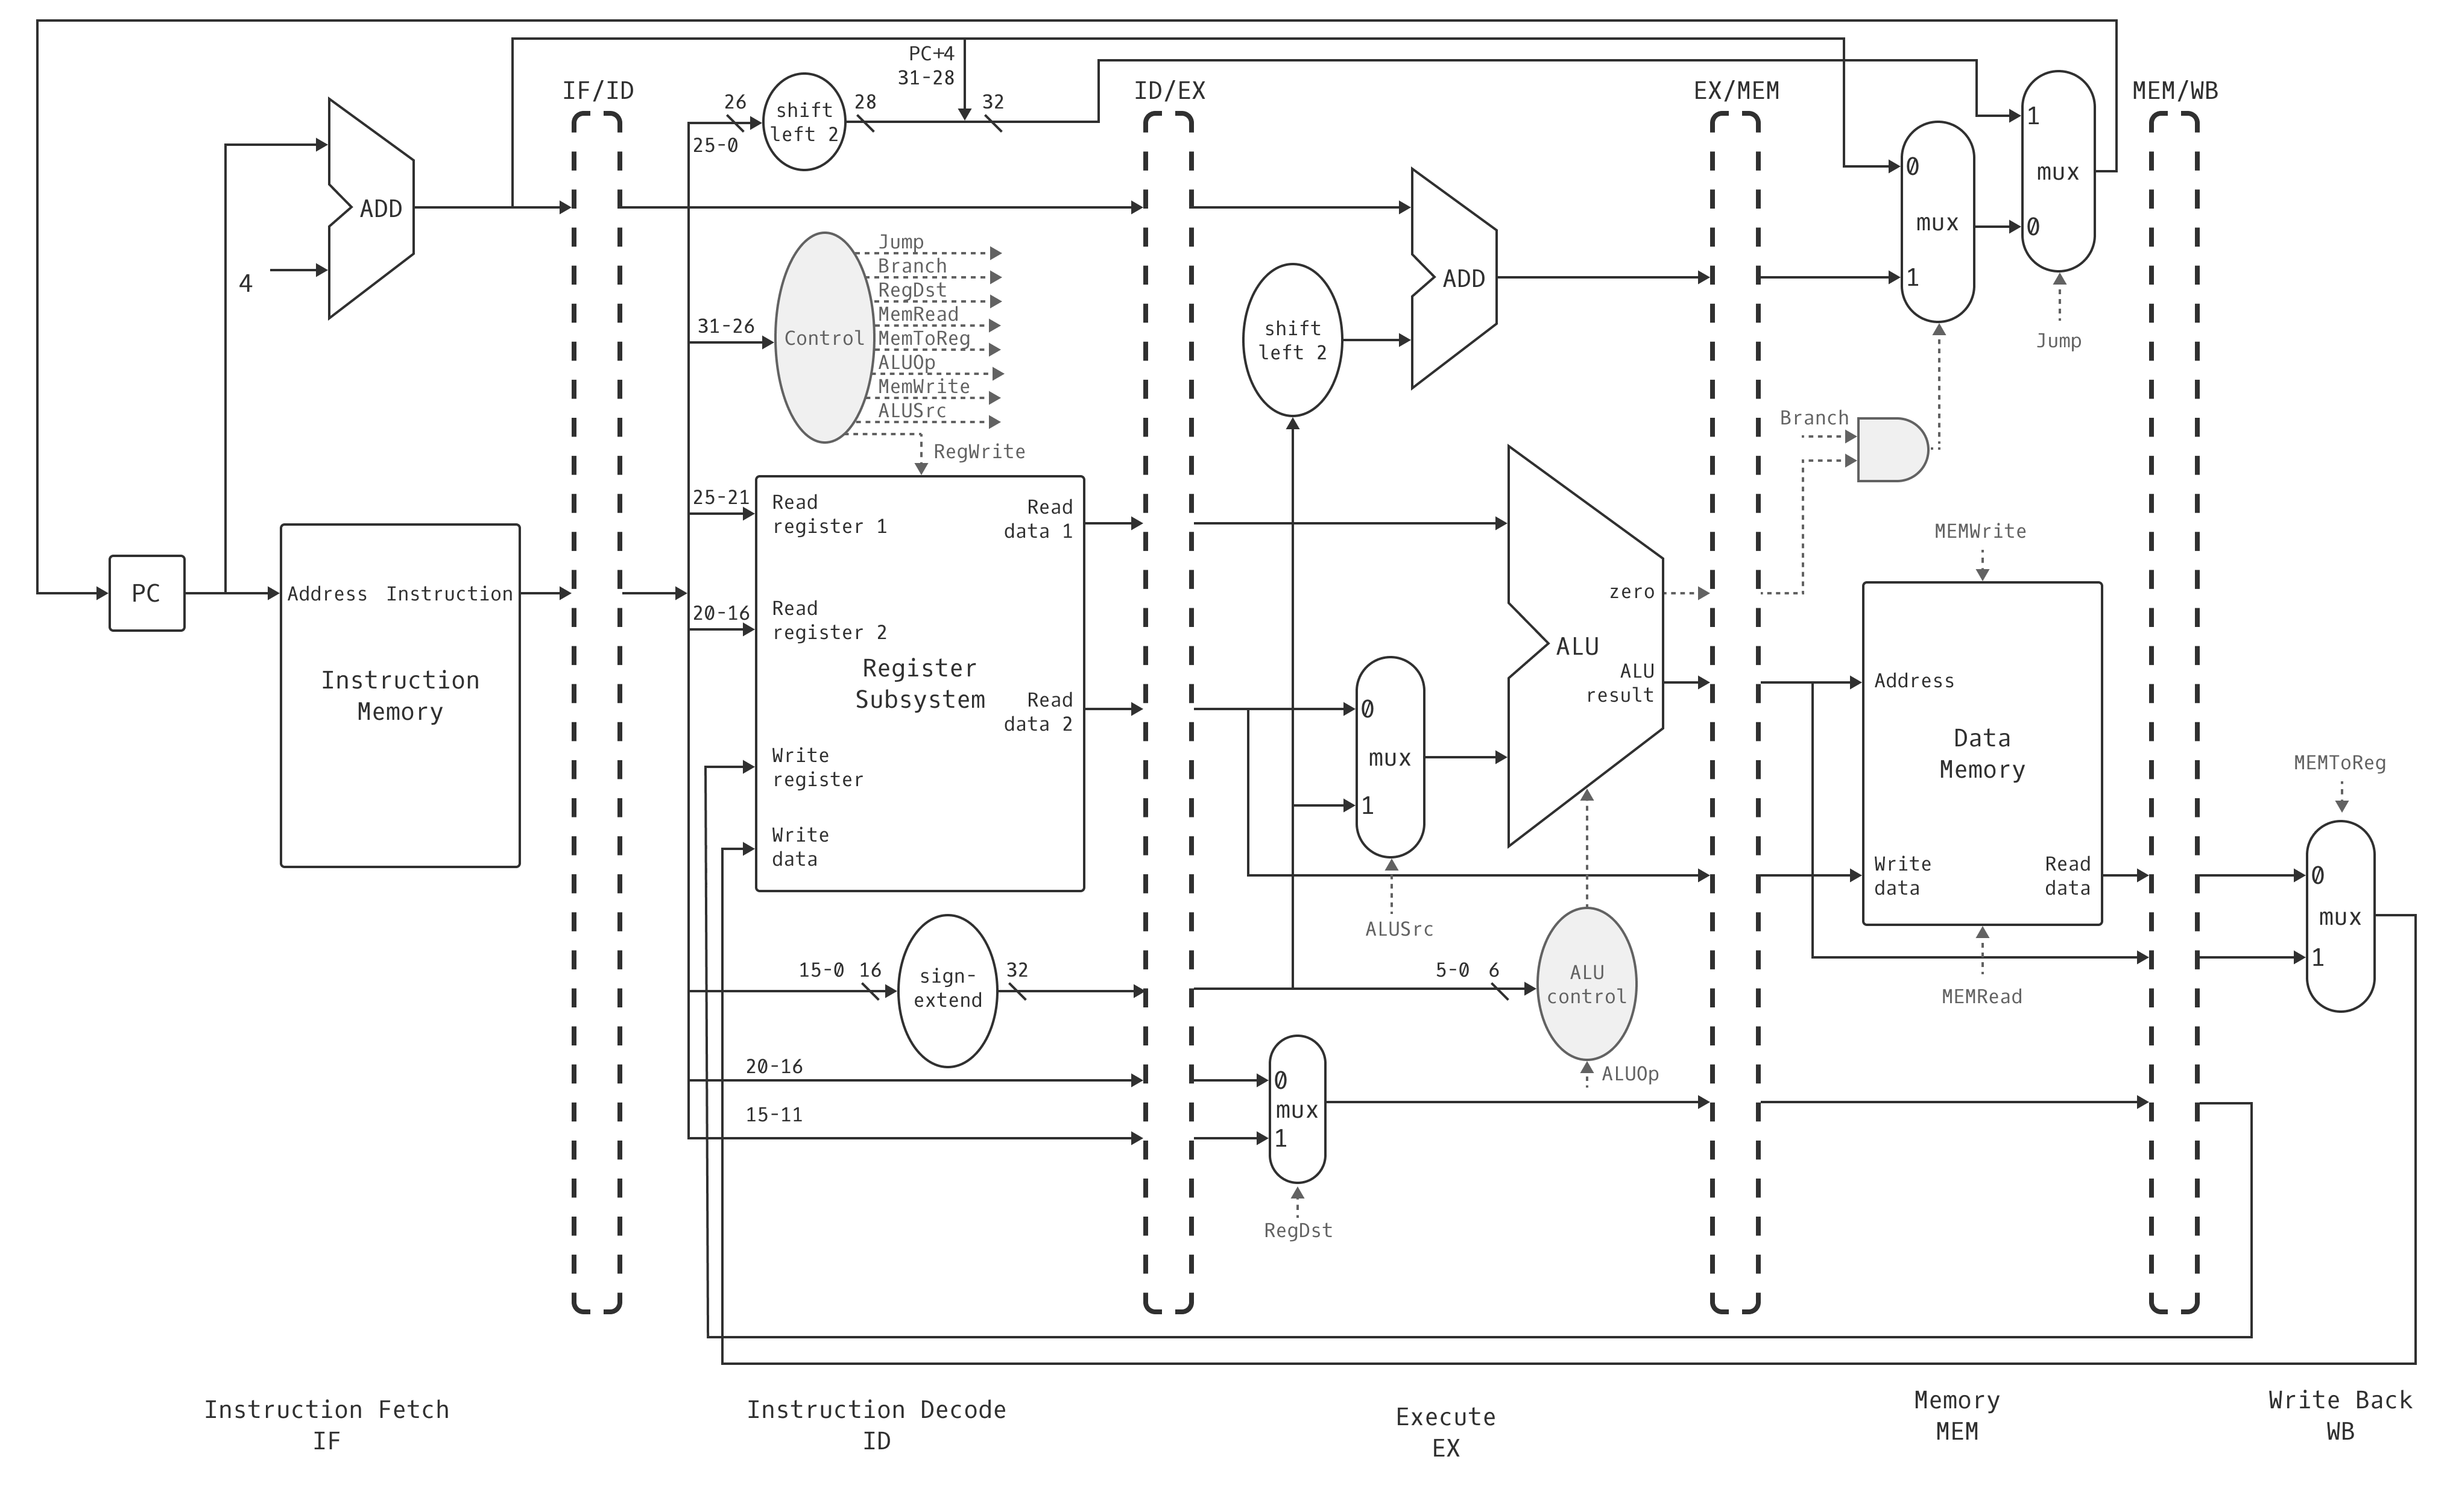
\includegraphics[width=1\textwidth]{assets/images/mips_pipeline_jump.png}
    \caption{High-Level MIPS Pipeline Diagram with Control Unit and Support for Unconditional Jump Instructions}
    \label{fig:mips_pipeline_jump}
\end{figure}

The only thing that was added was a multiplexer that selects the jump address from the ID stage if the instruction is a jump instruction. In this implementation the entirety of the jump executes in the ID stage. The jump address gets calculated, and the control unit generates the high $Jump$ control signal and immediately passes it to the multiplexer without going through the stage registers. This extended design will suffice for the purposes of explaining each instruction type execution in the pipeline which will be done in the next section.


\subsection{Example execution of each instruction type}
In this section, the execution of each instruction type in the MIPS pipeline will be discussed. This will include the subtypes of each instruction type, such as load and store instructions for the I-type format.

\subsubsection{R-type Instruction Execution}

\textbf{Arithmetic and logical R-type instructions}\newline 

\begin{verbatim}
    add $t0, $t1, $t2
\end{verbatim}
Machine format:
\begin{table}[H]
    \centering
    \begin{tabular}{|c|c|c|c|c|c|}
    \hline
    \textbf{opcode} & \textbf{rs} & \textbf{rt} & \textbf{rd} & \textbf{shamt} & \textbf{funct} \\ \hline
    0             & 9          & 10         & 8          & 0            & 32            \\ \hline
    \end{tabular}
    \caption{ADD Instruction Machine Format}
    \label{tab:add_instruction}
\end{table}

% Contriol signals
ADD Control signals:
% Table
\begin{table}[H]
    \centering
    \begin{tabular}{|c|c|}
    \hline
    \textbf{Control Signal} & \textbf{Value} \\ \hline
    ALUOp                   & 10             \\ \hline
    ALUSrc                  & 0             \\ \hline
    RegDst                  & 1             \\ \hline
    MemRead                 & 0             \\ \hline
    MemWrite                & 0             \\ \hline
    MemToReg                & 0             \\ \hline
    RegWrite                & 1             \\ \hline
    Branch                  & 0             \\ \hline
    Jump                 & 0             \\ \hline
    \end{tabular}
    \caption{Control Signals for ADD Instruction}
    \label{tab:add_control_signals}
\end{table}

As we can see the only control signals that are set to 1 is $RegWrite$, and $RegDst$. $RegWrite$ is set to 1 because we are writing to a register, and $RegDst$ is set to 1 because the destination register is in the rd field of the instruction. The $ALUOp$ is set to 10 to identify an R-type isntruction that has a funct field that we want to use as the operation to be performed by the ALU. $ALUSrc$ is set to 0 because we are not using an immediate value, and the ALU is getting its inputs from the register file. $MemRead$, $MemWrite$, $MemToReg$, $Jump$, and $Branch$ are all set to 0 because we are not reading or writing to memory, and we are not branching nor jumping.
First the instruction is fetched from memory and the next pc value is calculated by adding 4 to PC. Moving forward this value will be refered to as NPC(Next Program Counter). Then in the ID stage the control signals are generated, and the registers $t1$ and $t2$ are read from the register file. In the EX stage the ALU performs the addition operation and together with $t0$ the result is passed to the MEM stage. The MEM stage updates the PC to NPC and passes the ALU result from the EX stage to the WB stage, where it is written to register $t0$.

\textbf{Arithmetic and logical I-type instructions}\newline
\begin{verbatim}
    addi $t0, $t1, 100
\end{verbatim}
Machine format:
\begin{table}[H]
    \centering
    \begin{tabular}{|c|c|c|c|}
    \hline
    \textbf{opcode} & \textbf{rs} & \textbf{rt} & \textbf{imm} \\ \hline
    8             & 9          & 8          & 100          \\ \hline
    \end{tabular}
    \caption{ADDI Instruction Machine Format}
    \label{tab:addi_instruction}
\end{table}

% Control signals
ADDI Control signals:
% Table
\begin{table}[H]
    \centering
    \begin{tabular}{|c|c|}
    \hline
    \textbf{Control Signal} & \textbf{Value} \\ \hline
    ALUOp                   & 00             \\ \hline
    ALUSrc                  & 1             \\ \hline
    RegDst                  & 1             \\ \hline
    MemRead                 & 0             \\ \hline
    MemWrite                & 0             \\ \hline
    MemToReg                & 0             \\ \hline
    RegWrite                & 1             \\ \hline
    Branch                  & 0             \\ \hline
    MemWrite                 & 0             \\ \hline
    Jump                 & 0             \\ \hline
    \end{tabular}
    \caption{Control Signals for ADDI Instruction}
    \label{tab:addi_control_signals}
\end{table}

The control signals are the same as for the R-type instruction, except for $ALUSrc$ which is set to 1 because we are using an immediate value. The execution of the instruction is the same as for the R-type instruction, except that the ALU is performing an addition operation with an immediate value instead of a register value. Since this is an I-type instruction, there is no funct field for the ALU control unit to use. Therefore, the ALUOp signal is set to 00, which means that the ALU should perform an addition operation.

\textbf{Load and store instructions}\newline
\begin{verbatim}
    lw $t0, 100($t1)
    sw $t0, 100($t1)
\end{verbatim}

Machine format:
\begin{table}[H]
    \centering
    \begin{tabular}{|c|c|c|c|}
    \hline
    \textbf{opcode} & \textbf{rs} & \textbf{rt} & \textbf{imm} \\ \hline
    35             & 9          & 8          & 100          \\ \hline
    \end{tabular}
    \caption{Lw Instruction Machine Format}
    \label{tab:lw_instruction}

\end{table}

\begin{table}[H]
    \centering
    \begin{tabular}{|c|c|c|c|}
    \hline
    \textbf{opcode} & \textbf{rs} & \textbf{rt} & \textbf{imm} \\ \hline
    43             & 9          & 8          & 100          \\ \hline
    \end{tabular}
    \caption{Sw Instruction Machine Format}
    \label{tab:sw_instruction}

\end{table}


% Control signals
LW and SW Control signals:
% Table
\begin{table}[H]
    \centering
    \begin{tabular}{|c|c|c|}
    \hline
    \textbf{Control Signal} & \textbf{SW Value} & \textbf{LW Value} \\ \hline
    ALUOp                   & 00               & 00               \\ \hline
    ALUSrc                  & 1                & 1                \\ \hline
    RegDst                  & 0                & 1                \\ \hline
    MemRead                 & 1                & 1                \\ \hline
    MemWrite                & 1                & 0                \\ \hline
    MemToReg                & 0                & 1                \\ \hline
    RegWrite                & 0                & 1                \\ \hline
    Branch                  & 0                & 0                \\ \hline
    Jump                 & 0                & 0                \\ \hline
    \end{tabular}
    \caption{Control Signals for LW Instruction}
    \label{tab:lw_control_signals}
\end{table}

In the example of the $lw$ instructions, the control signals are the same as for the R-type instruction, except for $MemRead$ and $MemToReg$, which are set to 1 because we are reading from memory and writing the data to a register. Most of the execution is the same as for the R-type instruction.
The instruction gets fetched from memory, the registers $t1$ and $t0$ are read from the register file, and the ALU calculates the memory address by adding the immediate value to the value in register $t1$. The memory address is then passed to the MEM stage, where the data is read from memory and passed to the WB stage, where it is written to register $t0$.
Almost the same goes for the $sw$ instruction, except that the data is written to memory instead of being read from memory because of the $MemWrite$ control signal being set to 1 and the $MemToReg$ control signal being set to 0. And also nothing is written to the register file because of the $RegWrite$ control signal being set to 0.

\subsubsection{J-type Instruction Execution}
\begin{verbatim}
    j 100
\end{verbatim}

Machine format:
\begin{table}[H]
    \centering
    \begin{tabular}{|c|c|}
    \hline
    \textbf{opcode} & \textbf{addr} \\ \hline
    2             & 100          \\ \hline
    \end{tabular}
    \caption{J Instruction Machine Format}
    \label{tab:j_instruction}
\end{table}

% Control signals
J Control signals:
% Table
\begin{table}[H]
    \centering
    \begin{tabular}{|c|c|}
    \hline
    \textbf{Control Signal} & \textbf{Value} \\ \hline
    ALUOp                   & 00             \\ \hline
    ALUSrc                  & 0             \\ \hline
    RegDst                  & 0             \\ \hline
    MemRead                 & 0             \\ \hline
    MemWrite                & 0             \\ \hline
    MemToReg                & 0             \\ \hline
    RegWrite                & 0             \\ \hline
    Branch                  & 0             \\ \hline
    Jump                 & 1             \\ \hline
    \end{tabular}
    \caption{Control Signals for J Instruction}
    \label{tab:j_control_signals}
\end{table}

All the control signals are low except for the $Jump$ control signal which is set to 1. The execution of the jump instruction is quite simple and requires the least amount of hardware. This is visible in the section \ref{sec:jump_capabilities} where adding support for an unconditional jump instruction was explained. First the instruction gets fetched from memory, then the jump address is calculated in the ID stage, by shifting the 26-bit address left by 2 bits and concatenating the 4 most significant bits of the PC. The concatenation of the most significant bits of the PC is done so that the jump address is relative to current 256 MB segment of the PC value. Or more accurately, the jump address is relative to the address of the instruction following the jump instruction. And finally after the $Jump$ control signal is set, the multiplexer selects the jump address and the PC is updated to the jump address. All other stages are bypassed since the jump instruction doesn't require any other operations to be performed.




\section {Existing Solutions Analysis}

\subsection {Overview}\label{sec:existing_solutions_overview}
There are many simulators available for simulating the MIPS and other pipelines. Simulators like WinDLX\cite{grunbacher1996windlx}, VisualMIPS\cite{visualmips}, MARS\cite{mars}, WebMIPS, WebRISC-V\cite{Mariotti22-softwarex} just to name a few. However, the most important one in the context of this thesis is MIPSIM\cite{grunbacher1996windlx}, as it is the main inspiration and motivation for it. Even though it's the same concept, the simulators differ in their informativeness, user experience, feature set, and accessibility. These factors are arguably the most important when a simulator is chosen for educational purposes. The more informative a simulator is, the more can be learned from it. The better the user experience, the more focus will go into learning rather than figuring out how to use the simulator. The more features a simulator has, the more versatile it is in teaching different topics. And the more accessible a simulator is, the more students can use it.
If a simulator is a headache to use and doesn't provide enough information to the user, then it won't be very effective as a learning tool. In this section, the existing solutions will be analyzed based on these factors to see how they compare to each other.
But before that, the inspiration for this thesis, MIPSIM, will be briefly discussed.


\subsection{MIPSIM Case Study}

MIPSIM is a MIPS pipeline simulator that was developed by Herbert Grünbacher and Maziar Khosravipour at Vienna University of Technology. It is a MS-Windows (32 bit and 16 bit) based pipeline simulator for the MIPS processor which models a simple pipeline without hazard detection and forwarding units\cite{grunbacher1996windlx}. Much like the one described in section \ref{sec:mips_pipeline}.
\begin{figure}[H]
    \centering
    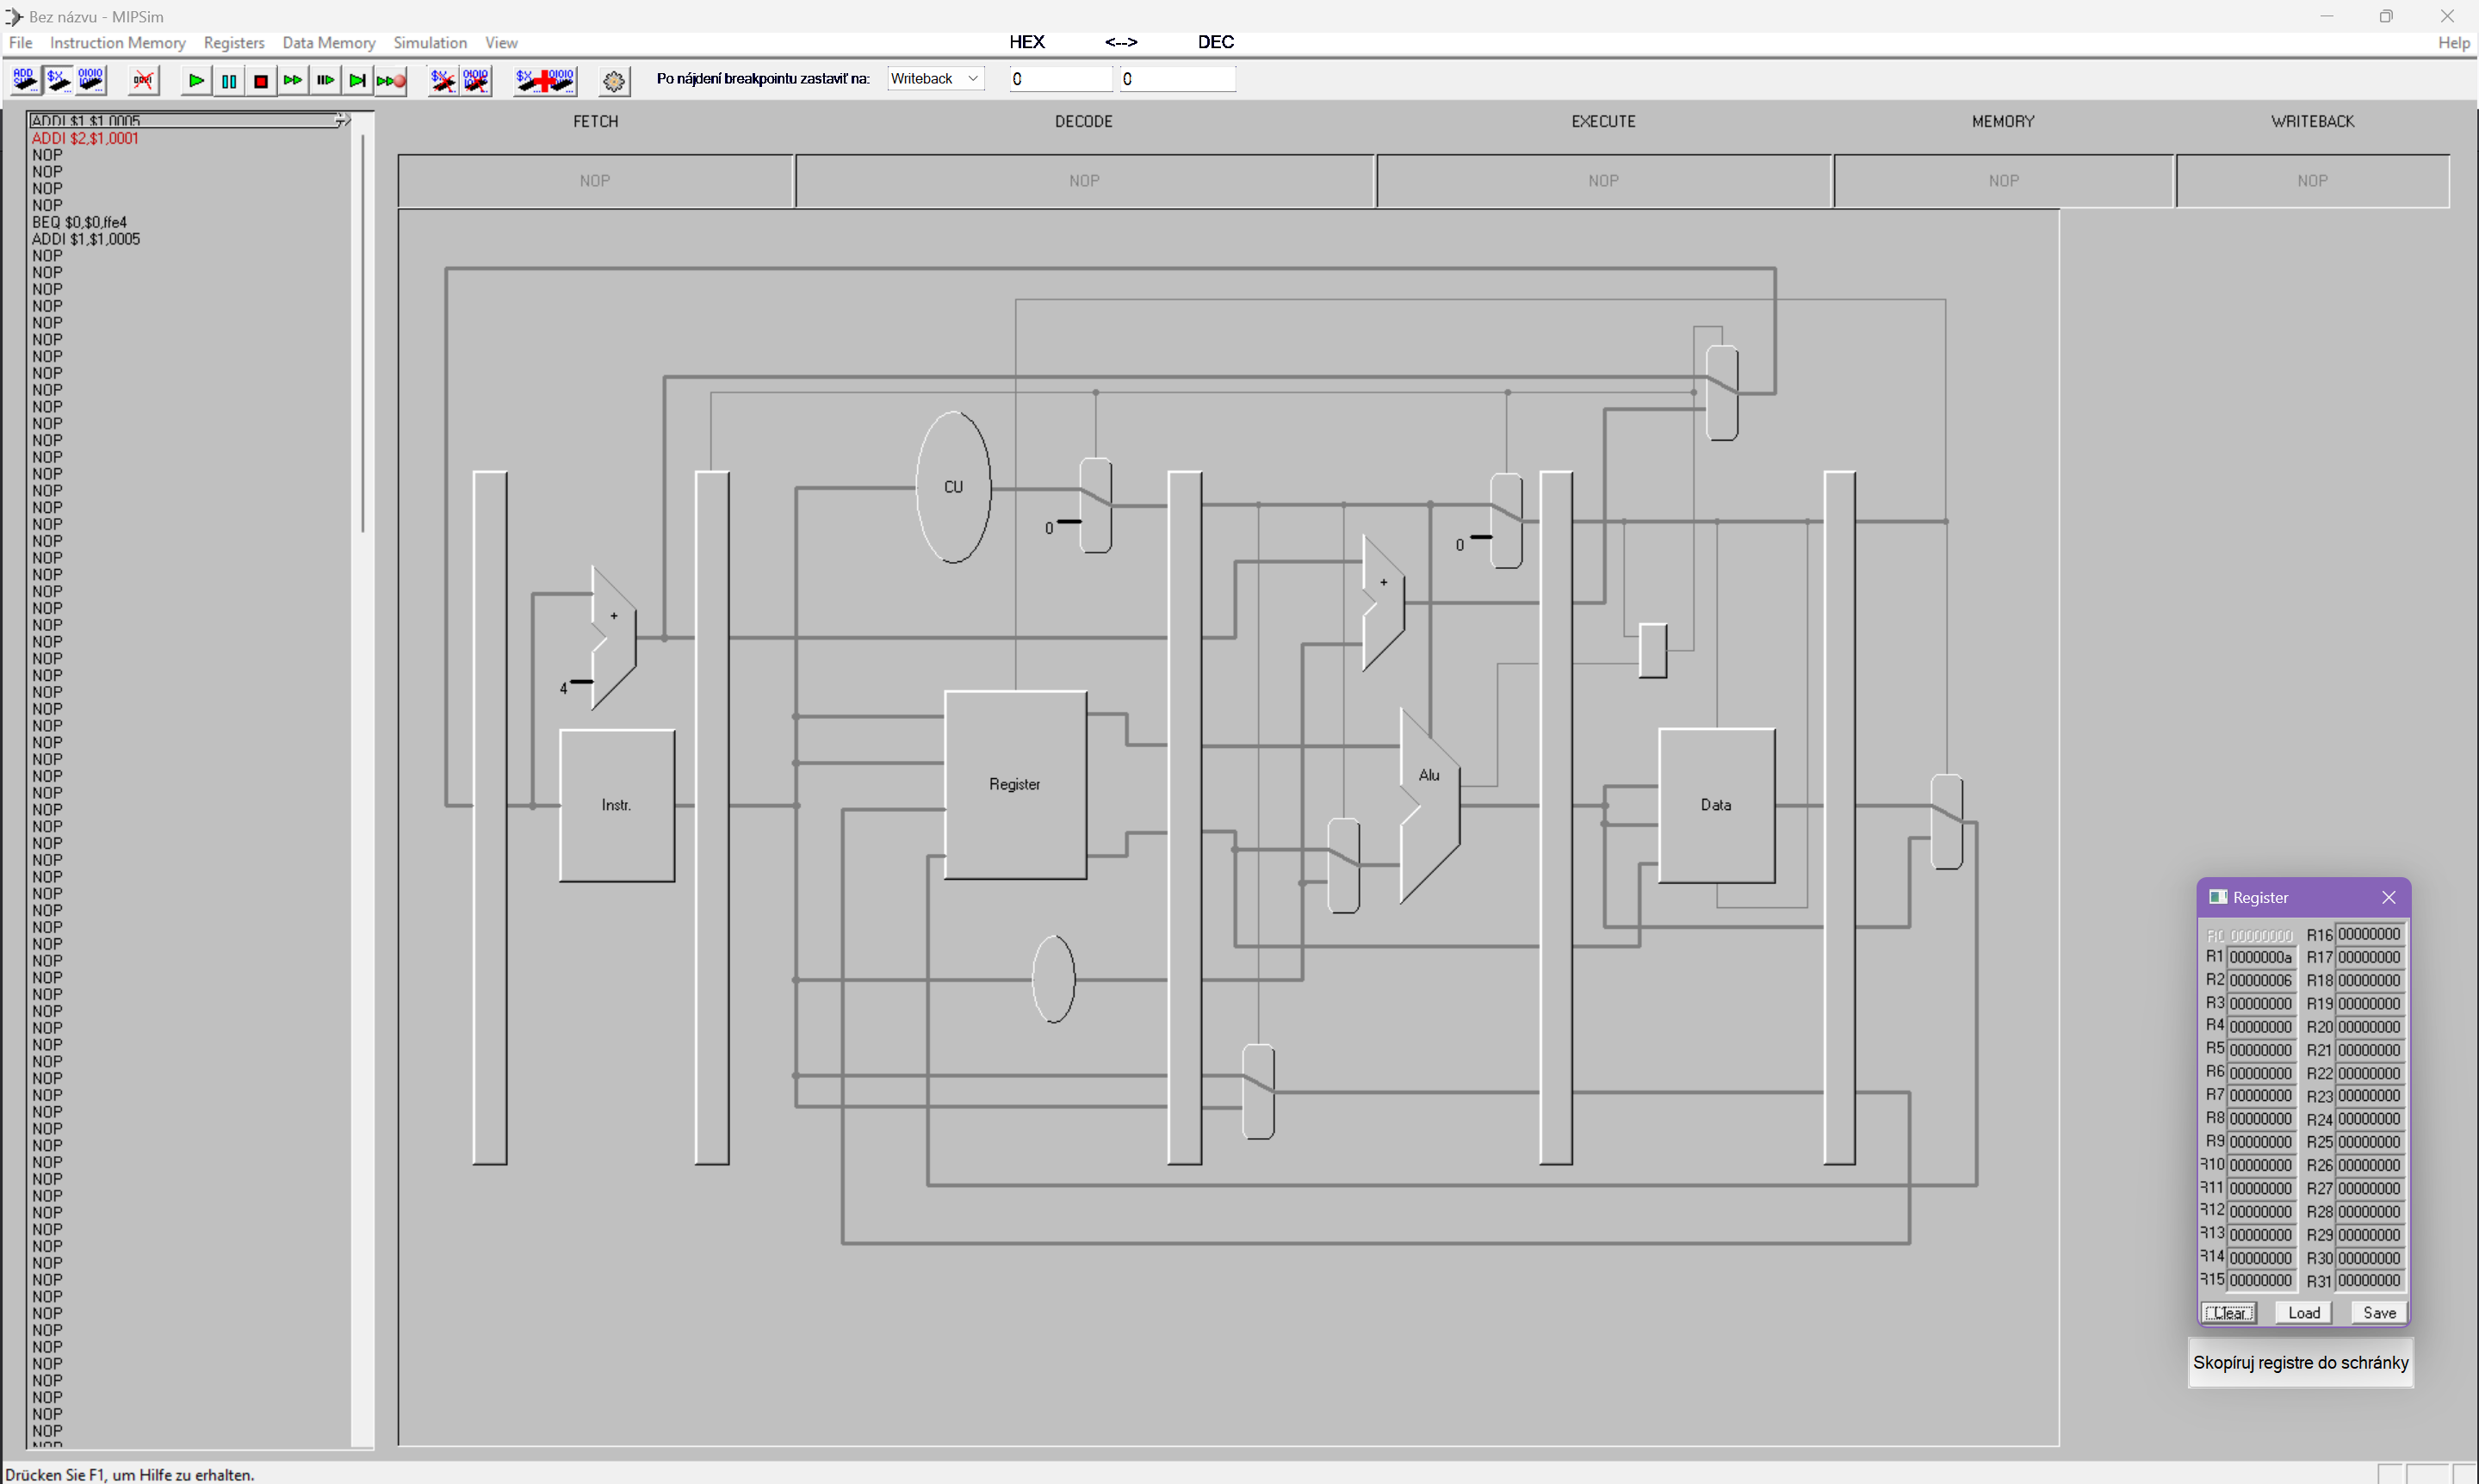
\includegraphics[width=1\textwidth]{assets/images/mipsim.png}
    \caption{MIPSIM User Interface with an Overlay Plugin}
    \label{fig:mipsim}
\end{figure}
Upon launching MIPSIM, one is greeted with a straightforward interface: the instruction memory on the left and a large pipeline diagram on the right. Additional windows for data memory and registers can be enabled as needed. Adding instructions is done via an icon that opens a new window, allowing the input of instructions. Memory, Register states, and instructions are editable and can be saved to their own file, adding a layer of flexibility. The execution controls are intuitive, featuring play, pause, stop, step, and skip-to-end buttons, making the simulation process simple to interact with.

However, the instruction window is where frustrations begin. Instructions are entered into rows, resembling a spreadsheet, but without any modern conveniences like syntax highlighting, autocomplete, or sanity checks. An instruction is either correct and saved, or incorrect and an error pops up preventing the user from doing anything before the instruction is correctly input. This lack of feedback is manageable, but the real headache comes when there is a need to reorder instructions. Unlike spreadsheet editors, MIPSIM offers no repositioning features. Moving an instruction means rewriting it as a NOP and then re-entering it in the desired position. This can be quite cumbersome, especially when trying to move multiple instructions or let alone the whole program, because an instruction needs to be inserted at the beginning of the program.

Despite these usability issues, the pipeline visualization is quite informative, clearly showing the datapaths used by each instruction. However, it falls short in labeling the inputs of various components, which can be confusing. 

Originally, MIPSIM lacked proper debugging support, and some features visible in Figure \ref{fig:mipsim} were added via an overlay plugin, which also enhances stability. In summary, MIPSIM is a simple, old, platform limited, somewhat cumbersome, yet sufficiently informative MIPS pipeline simulator that has served its purpose well, despite its quirks.


\subsection{Other Solutions Analysis}\label{sec:other_solutions_analysis}

Arguably, the most fundamental aspect of a pipelining simulator is the underlying processor design. Many simulators, including MIPSIM, are based on a straightforward MIPS pipeline design that often lacks hazard detection or forwarding units, or at least obscures these components. This is similar to the design described in section \ref{sec:mips_pipeline}. Numerous simulators, such as MIPS Visualizer, do not incorporate pipelining at all, opting instead for a single-cycle design limiting its feature set. Conversely, more sophisticated simulators like WebMIPS support both forwarding and hazard detection units, and even more sophisticated ones like DrMIPS allow the user to choose between different CPU designs.

However, regardless of the processor design, a simulator's educational value is significantly diminished without a user-friendly interface and informative features. WebMIPS excels in providing detailed information, displaying the bits of each machine instruction and the values of control signals. Unfortunately, its pipeline diagram is static and does not reflect the execution of instructions as MIPSIM or DrMIPS does, serving only as a visual aid. On the positive side, WebMIPS includes interactive elements that explain their functions when clicked, which is an excellent approach. This informativeness is very beneficial but also unfortunately, as is the case with WebMIPS, it can make the interface cluttered and hard to navigate. The interface of WebMIPS, while functional, may not be immediately intuitive, suggesting room for improvement despite a relatively shallow learning curve. 

DrMIPS on the other hand shows exactly what WebMIPS does, except that it tie everything together in a much more intuitive design including a reactive pipeline diagram. It also, as previously mentioned, features multiple cpu designs which is great for teaching purposes. Even though the interface has some quirks and possible minor improvements. The most major problem with DrMIPS is that it is Windows only, which is a big downside for students that use other operating systems.

That is where web based simulators come in to play. They are accessible to everyone on any device that supports a modern web browser, and they don't require any installation. WebRISC-V, WebMIPS, WeMIPS, VisualMIPS and a bunch of other web based simulators are great for this reason. Unfortunately none of them are as good as DrMIPS. The best out of the bunch is WebMIPS, but the issues mentioned before may be a dealbreaker for some students if not most students.

It would be important to mention that most simulators, such as VisualMIPS, WeMIPS, MARS, and SPIM, do not display a pipeline diagram, as they are not primarily designed as teaching tools. Nevertheless, they offer commendable user experience features. MARS, in particular, stands out as a robust and comprehensive simulator capable of testing real MIPS assembly code. It has a conventional and user-friendly interface that should be familiar to software engineering students, featuring syntax highlighting, autocomplete, and other functionalities that make writing code a breeze. Although MARS is not intended to teach the MIPS pipeline, its exceptional user experience makes it the best among the simulators reviewed.

Each simulator analyzed has its own strengths and weaknesses when it comes to educational use. While some excel in certain areas more than others, none of them are satisfactory in all aspects. If we could combine and adjust the features of all these simulators to meet the needs of students, we would have an ideal MIPS pipeline educational simulator. Better yet, a pipelining simulator that supports multiple architectures and offers a customizable feature set tailored to student requirements would be the ultimate solution.

% TODO: Reference all the simulators, fix the urls and add dates
\begin{itemize}
    \item MIPSIM\cite{grunbacher1996windlx}
    \item WinDLX\cite{grunbacher1996windlx}
    \item WebMIPS. (n.d.). Retrieved from \url{http://webmips.org}
    \item MARS (MIPS Assembler and Runtime Simulator). (n.d.). Retrieved from \url{http://courses.missouristate.edu/KenVollmar/mars/}
    \item DrMIPS. (n.d.). Retrieved from \url{http://drmips.org}
    \item WeMIPS. (n.d.). Retrieved from \url{http://wemips.org}
    \item MIPSim. (n.d.). Retrieved from \url{http://mipsim.org}
    \item WebRISC-V. (n.d.). Retrieved from \url{http://webriscv.org}
    \item VisualMIPS\cite{visualmips}
    \item SPIM
\end{itemize}

\subsection{MIPS pipeline simulator requirements}\label{sec:mips_pipeline_simulator_requirements}

From MIPSIM and from generally looking at the existing solutions, there are the minimum features that a MIPS pipeline simulator should have to be considered a minimum viable product. The most important ones would be the ability to input instructions, the ability to execute the instructions, and the ability to visualize the output of those instructions. But that wouldn't quite cut it if the simulator is supposed to also teach students about the MIPS pipeline. The more information the simulator provides about the execution of the instructions, the better. This includes the ability to see the values of the registers and the data memory, the ability to see the control signals, and the ability to see the values of the datapaths in the pipeline. The more information the simulator provides, the more effective it will be in teaching students about the MIPS pipeline and pipelining in general.


\section{Feature Analysis}\label{sec:feature_comparison}

In this section, the features that make up a MIPS pipeline simulator will be discussed, and the existing solutions will be compared based on those features.

\subsection{Instruction Input}\label{sec:instruction_input}
The ability to input instructions is the most basic feature that realistically any simulator or code execution environment should have. And for decades that has been the conventional text editor. Every simulator analyzed, except for MIPSIM has one. Some are basic like the one in WebMIPS, and some are more advanced like the one in MARS. Which one is better is subjective, but the more advanced the editor is, the easier it will be for students that can really take advantage of its additional features. And if something is unwanted, it can always be turned off.

\subsection{Instruction Execution}\label{sec:instruction_execution}
This is the feature that allows students execute their programs, a feature that every simulator has. Only thing that differs in each simulator are the execution controls. The most basic controls are play, pause, stop, and step, while more advanced controls would be the ability to set breakpoints, or the ability to change the speed of the execution. The more controls the better, but even the most basic ones are sufficient for the simulator to be effective.

\subsection{Visualization}\label{sec:instruction_visualization}
This is the feature that allows students to see what happened to the instructions they executed. This can range just from seeing the values of the registers and the data memory, to seeing the individual instruction going through the pipeline diagram. The visualization is the broadest feature, because there is so much that can be shown to the user. The more information the better, but the most basic information that should be shown is the values of the registers and the data memory, and the pipeline diagram. The pipeline diagram is the most important part of the visualization, because it shows the user how the instructions are executed, which is very important when it comes to teaching pipeline execution. WebMIPS, MIPSIM and DrMIPS are examples of simulators that have a pipeline diagram, with MIPSIM and DrMIPS actually show the instructions going through the pipeline, while WebMIPS just shows the pipeline diagram. DrMIPS actually has multiple cpu designs available, both single cycle and pipelined, and it shows the datapaths of the CPU, in each one. MARS, VisualMIPS, and SPIM are examples of simulators that don't have a pipeline diagram, but they do show the values of the registers and the data memory.

\subsection{Interactability}\label{sec:interactability}
Since the simulators should be analyzed from the perspective of a teaching tool, interactability is a very important feature. Poking around and observing changes is the single most effective way to learn about something. That even stems from the scientific method. The more interactive the simulator is, the more effective it will be in teaching students. The interactability can manifest itself in many ways. Editing a register value, creating custom instructions, or even just clicking on a component in the pipeline diagram to see what it does. A good example of this is WebMIPS and DrMIPS which have interactive elements that explain their functions when clicked. And most of the simulators have alterable data memory and register values, which is a good start. The more interactive the simulator is, the better.

\subsection{User Interface}\label{sec:user_interface}
User Interface is something that can make or break a simulator. It is the glue that holds everything together. If the user interface is bad, the simulator will be bad. The user interface should be intuitive, easy to use, and not cluttered. Example of a good user interface is MARS, which is simple, easy to use, and not cluttered. The user interface should also be customizable, so that the user can turn off features that they don't need, or turn on features that they do need. On the other spectrum is WebMIPS, which is very cluttered and a bit more difficult to navigate. 

\subsection{Accessibility}\label{sec:accessibility}
Accessibility plays a crucial role in the effectiveness of a teaching tool. The more accessible a simulator is, the broader its potential user base. Web-based simulators stand out in this regard, as they can be accessed from any device with a modern web browser, eliminating the need for installation. This makes them highly convenient for students who may be using different operating systems or devices. On the other hand, simulators that are limited to a single platform, such as Windows-only applications, restrict access to users with compatible devices. Among the simulators reviewed, WebMIPS, WebRISC-V, and WeMIPS are the most accessible due to their web-based nature. In contrast, MIPSIM and DrMIPS are less accessible, as they are confined to Windows environments.


\section{Analysis Conclusion}
This chapter has provided an overview of pipelining in general, went into the specifics of the MIPS architecture and its pipeline, and analyzed existing solutions and their features. The analysis has shown that while there are many simulators available, none of them are satisfactory in all aspects. Some simulators excel in certain areas, such as user experience or informativeness, but fall short in others. The most important features of a MIPS pipeline simulator have been identified, including instruction input, execution, visualization, interactability, user interface, and accessibility. A simulator that combines the best features of existing solutions and offers a customizable feature set tailored to student requirements would be the ultimate solution. The next chapter will introduce the design of the MIPS pipeline simulator, focusing on the features identified in this analysis.

% Solution Proposal
\clearpage\null
\chapter{Solution Proposal}
\label{chap:solution}
\section{Goals and Requirements}\label{sec:solution}
% Restate the main goals based on the problems found in the **Analysis**.  
To restate, the goal of this project is to create a modern instruction pipelining simulator that can be used to teach students about the concepts of pipelining and instruction execution in a CPU.

% Clearly define functional requirements (what the simulator must do).
\subsection{Functional Requirements}
\begin{itemize}
    \item Simulating a basic 5 stage instruction pipeline: Fetch, Decode, Execute, Memory Access, and Write Back is required.
    \item Support for a set of basic instructions (e.g., ADD, SUB, AND, OR, etc.) that can be executed in the pipeline is essential.
    \item An intuitive and responsive graphical user interface (GUI) should be provided for users to interact with the simulation. This includes simulation control(step forward, pause, reset), memory altering/display, register altering/display, code editor and a reactive pipeline diagram state visualization.
    \item Error handling for detecting and displaying of errors during the assembly of the program and or during the simulation. (e.g Syntax Errors, Division by zero errors, etc.)
    \item Cross-platform compatibility is required, allowing the simulator to run on different operating systems (Windows, macOS, Linux).
\end{itemize}
% Define non-functional requirements (performance, usability, scalability).
\subsection{Non-Functional Requirements}
\begin{itemize}
    \item Handle a reasonable number of instructions (e.g., up to 1000) without significant performance degradation.
    \item Support scalability, enabling future enhancements and additional features to be added without significant rework.
    \item Include comprehensive user manuals and documentation to assist users in understanding the simulator's functionality and usage.
    \item Ensure the simulator is lightweight and does not require excessive system resources, allowing it to run smoothly on a variety of hardware configurations.
    \item Undergo thorough testing to ensure reliability and correctness of the simulation results.
    \item Utilize a modular architecture, facilitating easy integration of new features and components in the future.
    \item Support multiple cpu architectures, allowing users to select different architectures for simulation.
\end{itemize}

\section{System Architecture}

Since the topic specification already defines that the project should be web-based for cross-platform compatibility, that direction will be followed. The simulator doesn't require a lot of resources, so it can be run on locally without the need for a external server. The simulator will be implemented as a single-page application (SPA) using Vue.js, a popular JavaScript framework for building user interfaces, to take advantage of its reactivity and component-based architecture. To store persistent data, such as projects or settings, indexDB will be used, which is a built-in database in modern browsers. This allows for the storage of data without the need for an external server or database. For simpler data storage if needed the localStorage API can be used, which is also built into modern browsers. 

This architecture allows for the project to be extended into a full-fledged desktop application with the use of electron or tauri software framework, which would allow the web app to be run as a native desktop application without the need for an internet connection. 

A modular breakdown of the application is shown in Figure \ref{fig:modular_breakdown}. The application will be divided into several modules, each responsible for a specific functionality. This modular approach allows for better organization of the code and makes it easier to add new features in the future.
% Use tikz to draw the diagram
\begin{figure}[H]
    \centering
    \begin{tikzpicture}[
        component/.style={rectangle, draw, rounded corners, minimum width=2.8cm, minimum height=1.1cm, align=center},
        subcomponent/.style={rectangle, draw, minimum width=2.5cm, minimum height=0.9cm, align=center},
        arrow/.style={->, thick},
        group/.style={draw, dashed, inner sep=0.2cm, rounded corners}
      ]
      
      % UI Layer
      \node (ui) [component] {User Interface};
      
      \node (simview) [subcomponent, below=0.2cm of ui, xshift=-4cm] {Simulator View};
      \node (projview) [subcomponent, below=0.2cm of ui,xshift=0cm] {Projects List View};
      \node (instview) [subcomponent, below=0.2cm of ui, xshift=4.7cm] {Instruction Config View};
      
      % Logic Layer
      \node (simengine) [component, below =of simview] {Simulation Engine};
      \node (projman) [component, below =of projview, ] {Project Manager};
      \node (custominst) [component, below =of instview] {Custom Instruction Manager};
      
      % CPU Layer
      \node (cpu) [component, below=2.2cm of simengine, xshift=0cm] {Pipeline CPU};
      \node (memory) [subcomponent, below=0.2cm of cpu, xshift=-2cm] {Memory};
      \node (registers) [subcomponent, below=0.2cm of cpu, xshift=2cm] {Registers};

      \node (assembler) [component, below=0.5cm of simengine, xshift=-2cm] {Assembler};
      
      \node[fit=(cpu)(memory)(registers), group, label=below:CPU Model] {};
      
      % Storage Layer
      \node (storage) [component, below=1.2cm of custominst, xshift=-0.4cm] {Storage};
      \node (proj) [subcomponent, below=0.5cm of storage, xshift=-2.8cm] {Projects};
      \node (instdata) [subcomponent, below=1.5cm of storage] {Custom Instructions};
      \node (settings) [subcomponent, below=0.5cm of storage, xshift=2.5cm] {Settings};
      
      % Connections UI -> Logic
      \draw[arrow] (simview.south) -- (simengine.north);
      \draw[arrow] (instview.south) -- (custominst.north);
      
      % UI -> Storage for Projects
      \draw[arrow] (projview.south) -- (projman.north);
      \draw[arrow] (projman.south) -- (storage.north);
      
      % Logic Layer connections
      \draw[arrow] (simengine.south) -- (assembler.north);
      \draw[arrow] (simengine.south) -- (cpu.north);
      \draw[arrow] (simengine.east) -- (projman.west);
      \draw[arrow] (simengine.south) -- (storage.west);
      \draw[arrow] (custominst.south) -- (storage.north);
      
      % CPU internals
      \draw[arrow] (cpu.south west) -- (memory.north);
      \draw[arrow] (cpu.south east) -- (registers.north);
      
      % Storage subcomponents
      \draw[arrow] (storage.south) -- (proj.north);
      \draw[arrow] (storage.south) -- (settings.north);
      \draw[arrow] (storage.south) -- (instdata.north);
      
      \end{tikzpicture}
      \caption{High-level Modular Breakdown of the Simulator's Architecture}
    \label{fig:modular_breakdown}
\end{figure}


\subsection{User Interface Layer}
The User Interface (UI) layer is the main interaction point between the user and the simulator. It consists of three views:

1. \textbf{Simulator View}: Displays the pipeline diagram, memory, registers, and controls for starting, pausing, stepping, and resetting the simulation.

2. \textbf{Projects List View}: Manages simulation projects with options to create, open, rename, delete, and search projects. Integrates with IndexDB for data persistence.

3. \textbf{Instruction Configuration View}: Allows customization of the instruction set, including adding, editing, and validating instructions. Ensures proper definition before adding them to the simulator.

\subsection{Logic Layer}
The Logic Layer handles the simulator's core functionality, comprising the Simulation Engine, Project Manager, and Custom Instruction Manager.

The Simulation Engine executes the instruction pipeline, updates the pipeline diagram, and interfaces with the Assembler and CPU model.

The Project Manager manages simulation projects, including creation, loading, saving, and deletion, while interacting with IndexDB for data persistence.

The Custom Instruction Manager enables users to define, edit, and validate custom instructions, extending the simulator's instruction set and at the same time learning how instructions are defined and how they work.

\subsection{Assembler}
The Assembler is responsible for converting assembly code into machine code that can be executed by the simulation engine. It parses the assembly code, identifies labels, resolves addresses, and generates the corresponding machine code instructions. The Assembler should also perform error checking to ensure that the assembly code is valid and provides feedback to the user in case of syntax errors or other issues.

\subsection{CPU Model}
The CPU Model represents the simulated pipeline CPU architecture. It consists of the Pipeline CPU, which implements the classic 5-stage instruction pipeline (IF, ID, EX, MEM, WB), and the Memory and Registers components. The CPU Model is responsible for executing instructions, managing data flow between stages and depending on the model, it may also include features like hazard detection and forwarding to handle data hazards.

\subsection{Storage Layer}
The Storage Layer is responsible for persisting user data, including projects, custom instructions, and settings. While IndexDB is the primary storage mechanism due to its ability to handle structured data and larger datasets, localStorage may also be utilized for simpler, temporary data storage needs, such as caching user preferences or session-specific data. This dual approach ensures flexibility and efficiency in managing data storage requirements.





\section{Pipeline Simulation Model}
The pipeline simulation model will be based on a classic 5-stage instruction pipeline, which was already discussed in the \ref{sec:analysis} section. The stages of the pipeline are IF (Instruction Fetch), ID (Instruction Decode), EX (Execute), MEM (Memory Access), and WB (Write Back). It will also include register and memory arrays, which will be used to store the state of the CPU during the simulation.

Inorder to implement multiple CPU models in the future, the CPU model has to be designed in a modular way, allowing for easy integration of new models. Ideally as a class that will have a standardized interface for all CPU models. This will allow for easy switching between different CPU models without having to change the underlying code of the simulator. 

Instruction set and control signals will be defined in the CPU model, which will be used by the assembler to assemble the instructions into machine code and by other parts of the simulator to execute the instructions.

Simulating the pipeline is an intriguing challenge, as in the real world, each component in the pipeline performs its task independently and concurrently. While, unfortunatly, JavaScript is single-threaded(except for Web Workers which would be impractical to use), and therefore the pipeline execution will be simulated in a sequential manner. Luckily, simulating the pipeline sequentially from the WB stage to the IF stage is a good approximation of how the pipeline would work in a real CPU and avoids any dependency issues. 

\section{Instruction Set Model}
Before the pipeline can be simulated, instructions need to be assembled into machine code. And to make the instruction set extensible, there needs to be a configuration for each instruction. This configuration will include the following fields:
\begin{table}[H]
    \centering
    \begin{tabular}{|l|l|l|}
        \hline
        \textbf{Field} & \textbf{Type} & \textbf{Description} \\ \hline
        opcode & number & The opcode of the instruction. \\ \hline
        mnemonic & string & The mnemonic of the instruction. \\ \hline
        type & InstructionType & The type of the instruction (R-Type, I-Type, J-Type). \\ \hline
        description & string & A short description of the instruction. \\ \hline
        controlSignals & object & The control signals for the instruction. \\ \hline
        funct & number & The funct field for R-Type instructions. \\ \hline
        operands & OperandType[] & The operands for the instruction (Rs, Imm, label, etc...). \\ \hline
    \end{tabular}
    \caption{Instruction Configuration Fields}
    \label{tab:instruction_config}
\end{table}

These fields will be used to define each instruction in the instruction set and will be stored in a JSON object. Each CPU should have their own default instruction set, which can be extended by the user. The instruction set will be stored in the CPU model and will be used by the assembler to assemble the instructions into machine code.

\section{User Interface \& Interaction}

As mentioned before. The entirety of the simulator will be implemented as a single-page application (SPA) using Vue.js. The individual pages or views will be implemented as Vue components, which will be responsible for rendering the UI and handling user interactions. 

\section{Project Lists Page}

The projects list will be the home page of the application, which will display a list of projects that the user has created. The user can create a new project, open an existing project, or delete a project from this page. The projects will be shown as a simple table with the project name, last modified date, and a button to open the project. The user can also search for projects by name or filter them by date.

\begin{figure}[H]
    \centering
    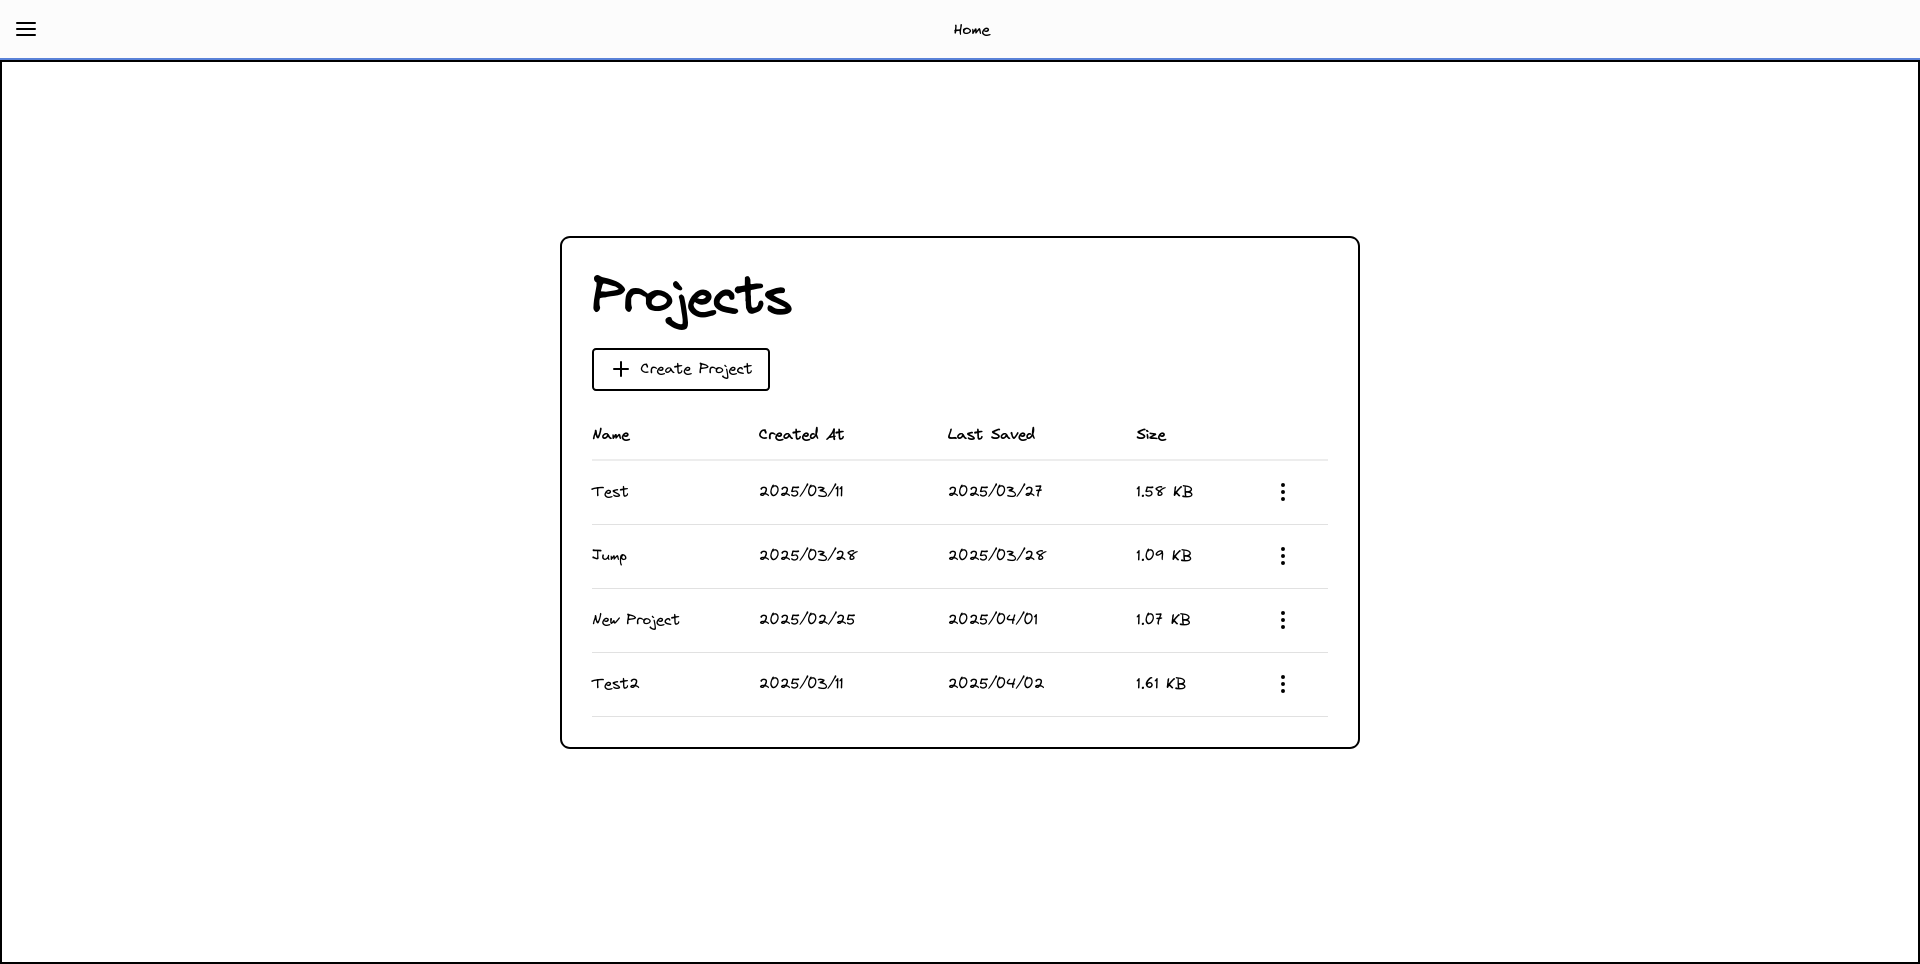
\includegraphics[width=1\textwidth]{assets/images/projects_list_wireframe.png}
    \caption{Wireframe of the Projects List Page}
    \label{fig:projects_list_wireframe}
\end{figure}

\section{Instruction Configuration Page}
The instruction configuration page enables users to define custom instructions for the simulator. Users can add, edit, or delete instructions directly from this page. Since each processor architecture has its own unique instruction set, users must first select the architecture they wish to configure. Once selected, a list of default instructions for the chosen architecture, along with any custom instructions previously defined by the user, will be displayed. Further on that will be a section for editing the selected instruction, which will include all the fields defined in Table \ref{tab:instruction_config}. 



\begin{figure}[H]
    \centering
    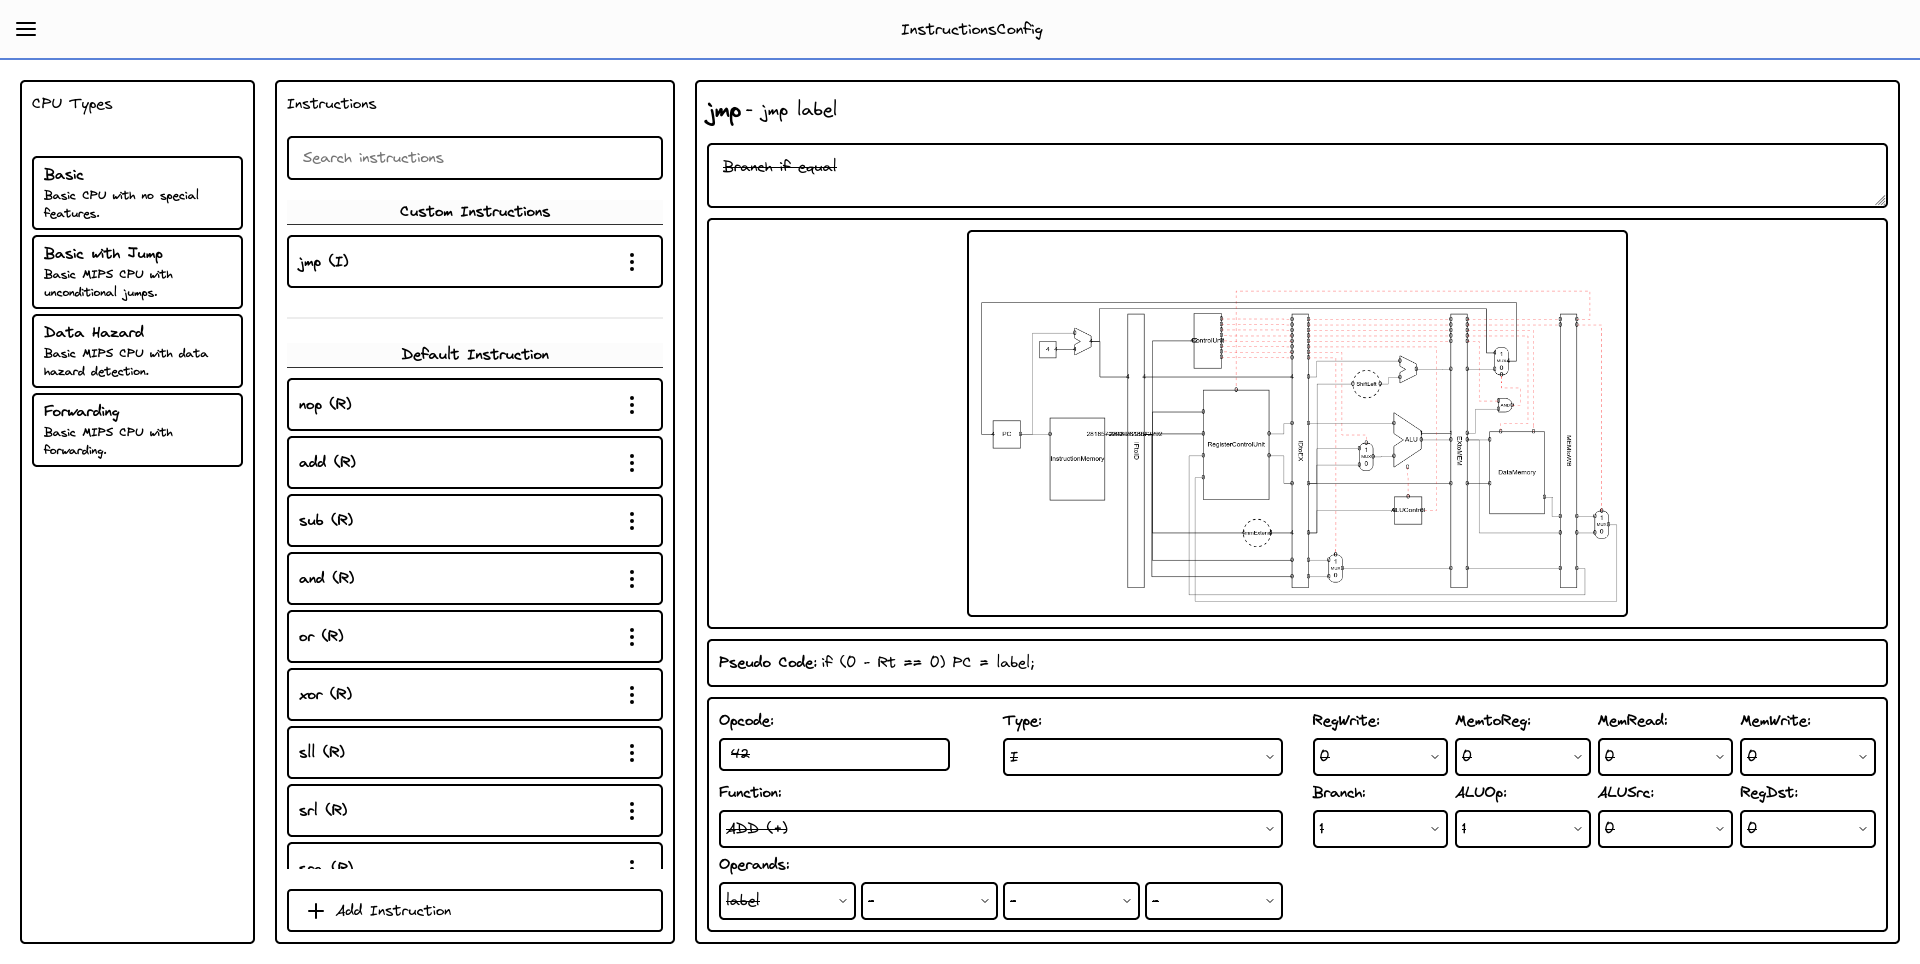
\includegraphics[width=1\textwidth]{assets/images/instruction_config_wireframe.png}
    \caption{Wireframe of the Instruction Configuration Page}
    \label{fig:instruction_config_wireframe}
\end{figure}

\section{Simulator Page}
The simulator page serves as the primary interface of the application, showcasing the pipeline diagram, memory, registers, and controls for managing the simulation (start, pause, step, and reset). Each component, including the pipeline diagram, editor, memory, and registers, will be movable and resizable, allowing users to customize the layout to their preference. The pipeline diagram will take center stage, providing a visual representation of the pipeline's current state and the instructions being executed. Memory and registers will be displayed in a straightforward table format, reflecting their current states. Controls for managing the simulation will be positioned above the editor. The problems tab will display any errors or warnings, and additionally, a searchable instruction list will be available, showing all instructions currently loaded into the simulator.

\begin{figure}[H]
    \centering
    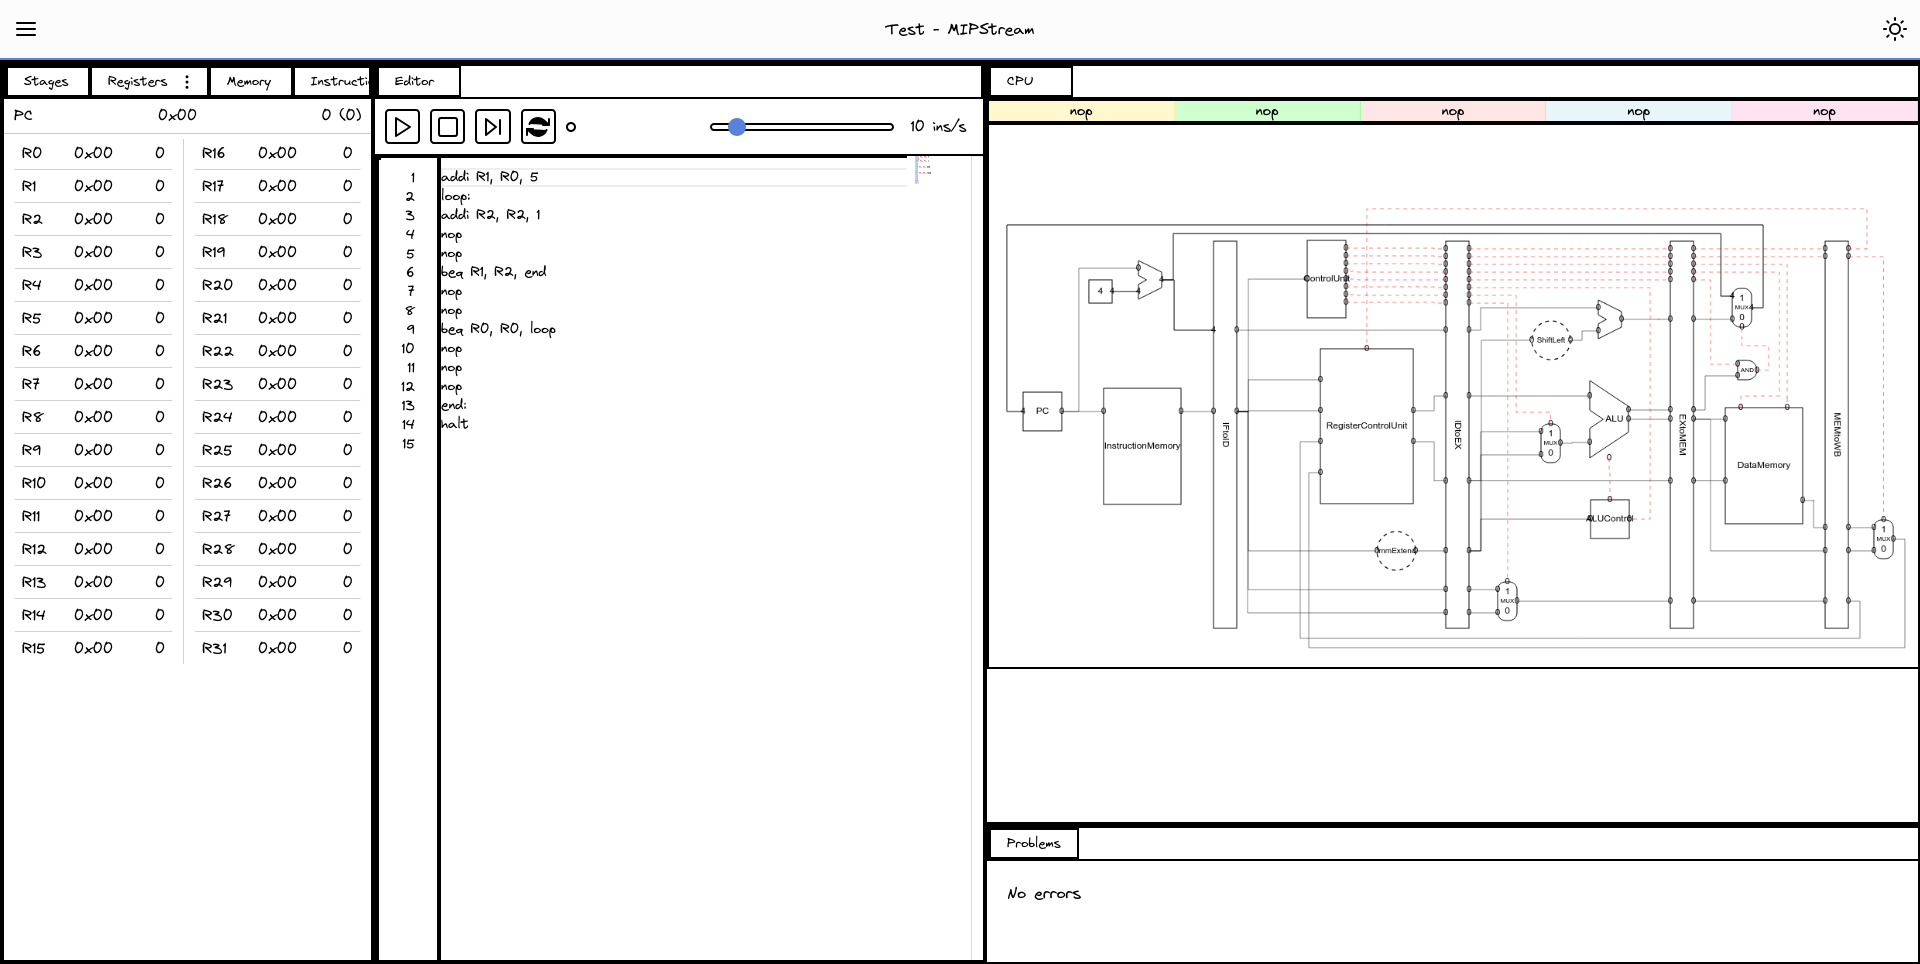
\includegraphics[width=1\textwidth]{assets/images/simulator_wireframe.png}
    \caption{Wireframe of the Simulator Page}
    \label{fig:simulator_wireframe}
\end{figure}


\subsection{Editor}
For a simple and feature-full implementation of an editor for the assembly code, the Monaco Editor will be used. It is a powerful code editor that is based on Visual Studio Code's editor. It supports syntax highlighting, code completion, error checking, and many other features that are essential for a code editor. The Monaco Editor is also highly customizable, allowing for the addition of custom themes, keybindings, and other features. It is also lightweight and fast, making it ideal for a web-based application.

\subsection{Pipeline Diagram}
The pipeline diagram should be implemented using the Canvas API. The Canvas API is a powerful and flexible way to draw graphics on the web. It allows for the creation of complex shapes, animations, and interactions. The Canvas API is also highly performant, making it ideal for a simulation application. The pipeline diagram will be drawn on a canvas element, which will be updated in real-time as the simulation progresses. This will allow for a smooth and responsive user experience. 
As opposed to using SVG, which is a markup language for describing two-dimensional graphics, implementing the diagram with the Canvas API will be more time-consuming and complex in the short term. But when it comes to ease of adding other features and more diagrams for different CPU architectures, the Canvas API will be a much better choice in the long run.

The pipeline diagram will work by receiving a configuration of the components and connections, then drawing them. This makes it easier to edit the diagram as it will have a specially designed logic for this use case. To update its state, it should ideally be tied directly to the cpu's state, so that it can be updated in real-time. This will allow for a smooth and responsive user experience. Hovering over any component or port should trigger an information box popup that will show the current state of the component or port. And the values of each port should be displayed in the diagram, so that the user can see the current state of the pipeline at a glance.

% Figure
\begin{figure}[H]
    \centering
    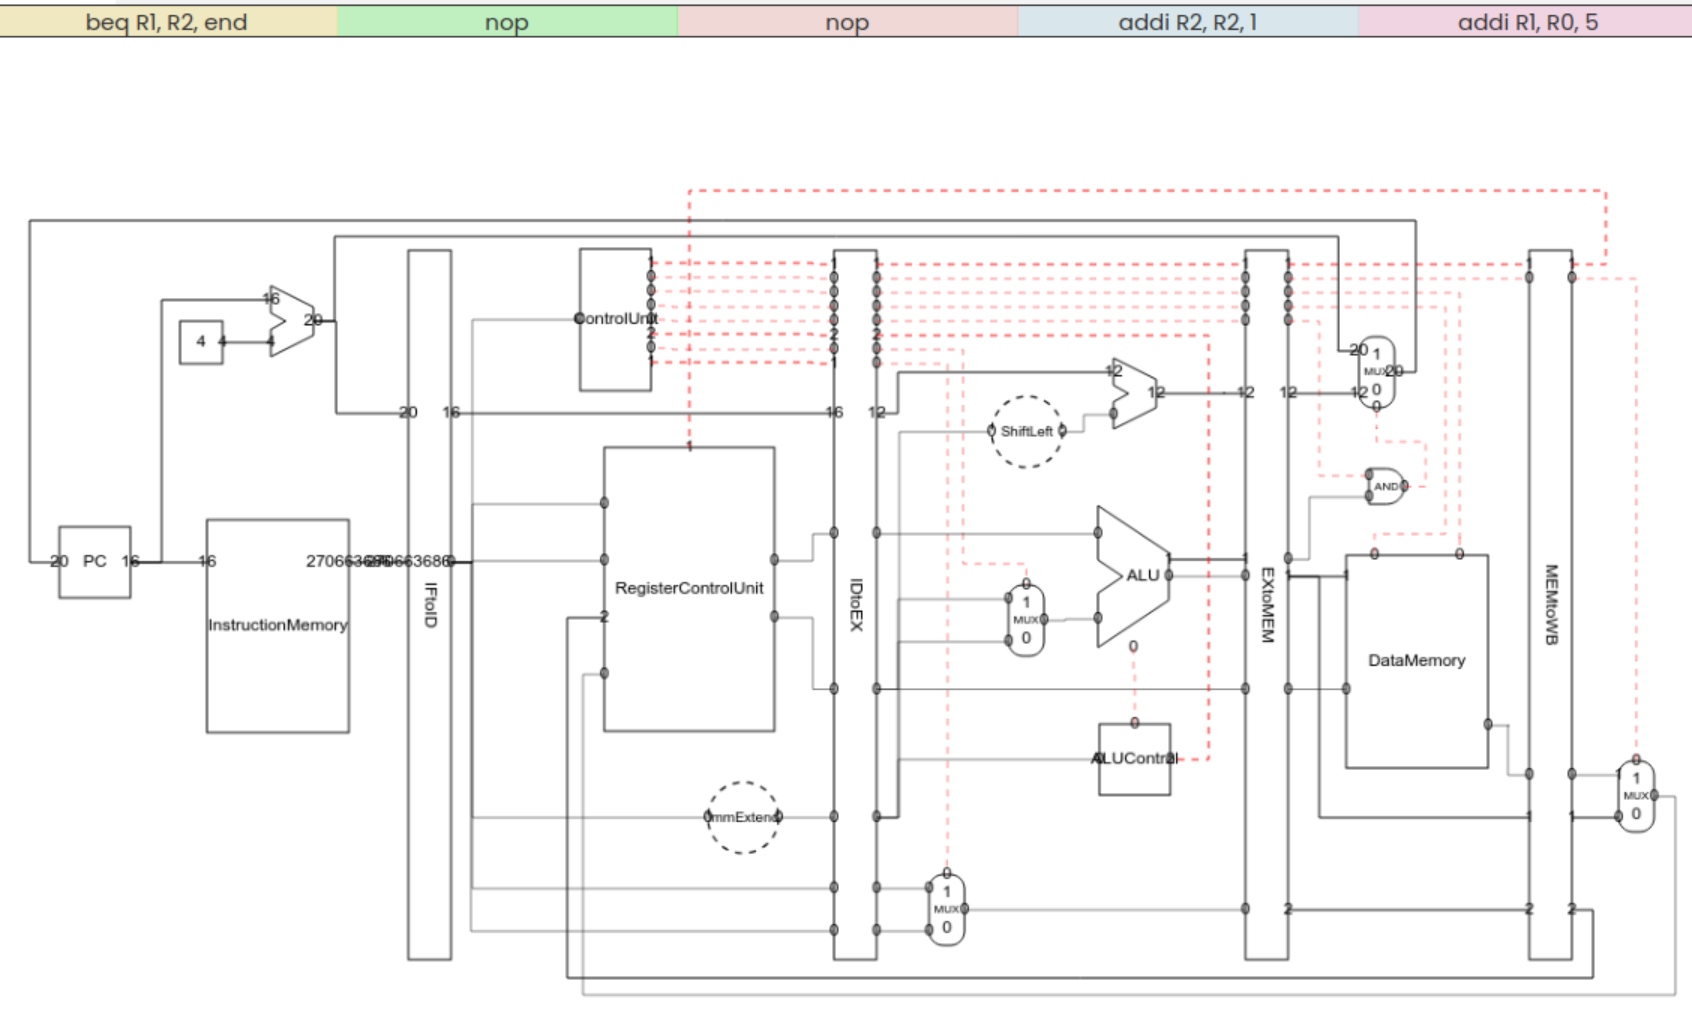
\includegraphics[width=1\textwidth]{assets/images/pipeline_diagram_example.png}
    \caption{Example of a Pipeline Diagram}
    \label{fig:pipeline_diagram_example}
\end{figure}

\subsection{Memory and Register Display}
The memory and register display should both be implemented as a simple table that shows the current state of the memory and registers. The table should be updated in real-time as the simulation progresses, so that the user can see the current state of the memory and registers at a glance. The table should also allow for editing of the values when clicking on them, so that the user can modify the state of the memory and registers during the simulation. This will allow for a more interactive and engaging user experience.

\subsection{Error Handling}
Error handling is an important part of any application, and the simulator is no exception. The simulator should be able to handle errors gracefully and provide feedback to the user in case of errors. This includes syntax errors in the assembly code, invalid instructions, and other errors that may occur during the simulation or assembly. The error handling should be implemented in a way that allows for easy debugging and troubleshooting. The error should be shown both in the editor at the line where the error occurred and in a separate error log that shows all errors.

\subsection{Settings}
The settings will be accessible through the top-left hamburger menu of the application. They should be presented as a straightforward form, enabling users to customize various aspects of the simulator. This includes selecting the default CPU model, adjusting UI themes, and configuring other relevant preferences. The settings will be saved in the browser's local storage, ensuring they persist across sessions and provide a consistent user experience.




% Solution Proposal
\clearpage\null
\chapter{Implementation}

% Solution Verification
\clearpage\null
\chapter{Solution Verification}

\lipsum


% % Evaluation
% \clearpage\null
% \chapter{Evaluation \label{cha:eva}}

\lipsum


% % Related Work
% \clearpage\null
% \chapter{Related Work}


% Conclusion
\clearpage\null
\chapter{Conclusion}

\section{Summary}


\section{Future Work}


% Resume
\clearpage\null

\chapter*{Resumé}

\lipsum

% Bibliography
\clearpage\null
\printbibliography[heading=references,segment=\therefsegment,resetnumbers=true]

\end{refsegment}

% Appendix
\appendix

\clearpage\null
\setcounter{figure}{0}
\setcounter{listing}{0}

\chapter{First Appendix \label{cha:chapter1} }

\begin{refsegment}

% Appendix
% \chapter{Second Chapter}

\say{Here, a quotation is written and even some \say{nested} quotations 
are possible}

\lipsum

Figure \ref{fig:dynabook}:

\begin{figure}[h]
\begin{centering}
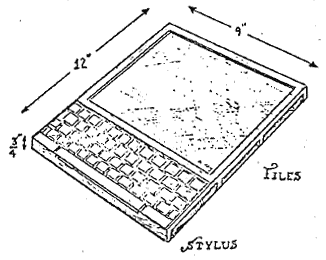
\includegraphics[width=5cm]{assets/images/Dynabook}
\par\end{centering}
\caption{Dynabook \label{fig:dynabook}}
\end{figure}

% Bibliography
\printbibliography[heading=referencessec,segment=\therefsegment,resetnumbers=true]

\end{refsegment}

\clearpage\null
\chapter{Contents of Included CD–ROM \label{cha:cdrom} }

CD–ROM included to the thesis contains following files:

\begin{itemize}
\item \texttt{/file1} --- First file
\item \texttt{/file2} --- Second file
\end{itemize}


\end{document}
